\section{Double-differential cross-sections from reaction of p+Nb at 3.5 GeV}

The double differential cross-section for production of charged pions and isotopes of hydrogen in p+Nb reaction at 3.5 GeV proton beam energy resulting from the analysis of data registered in HADES experiment are shown in figs. \ref{Protonall}, \ref{pdt_all} and \ref{pi_all}. These distributions are effect of the analysis explained in chapter \ref{chapter:3}.

\begin{figure}[!hbt]
\centering
	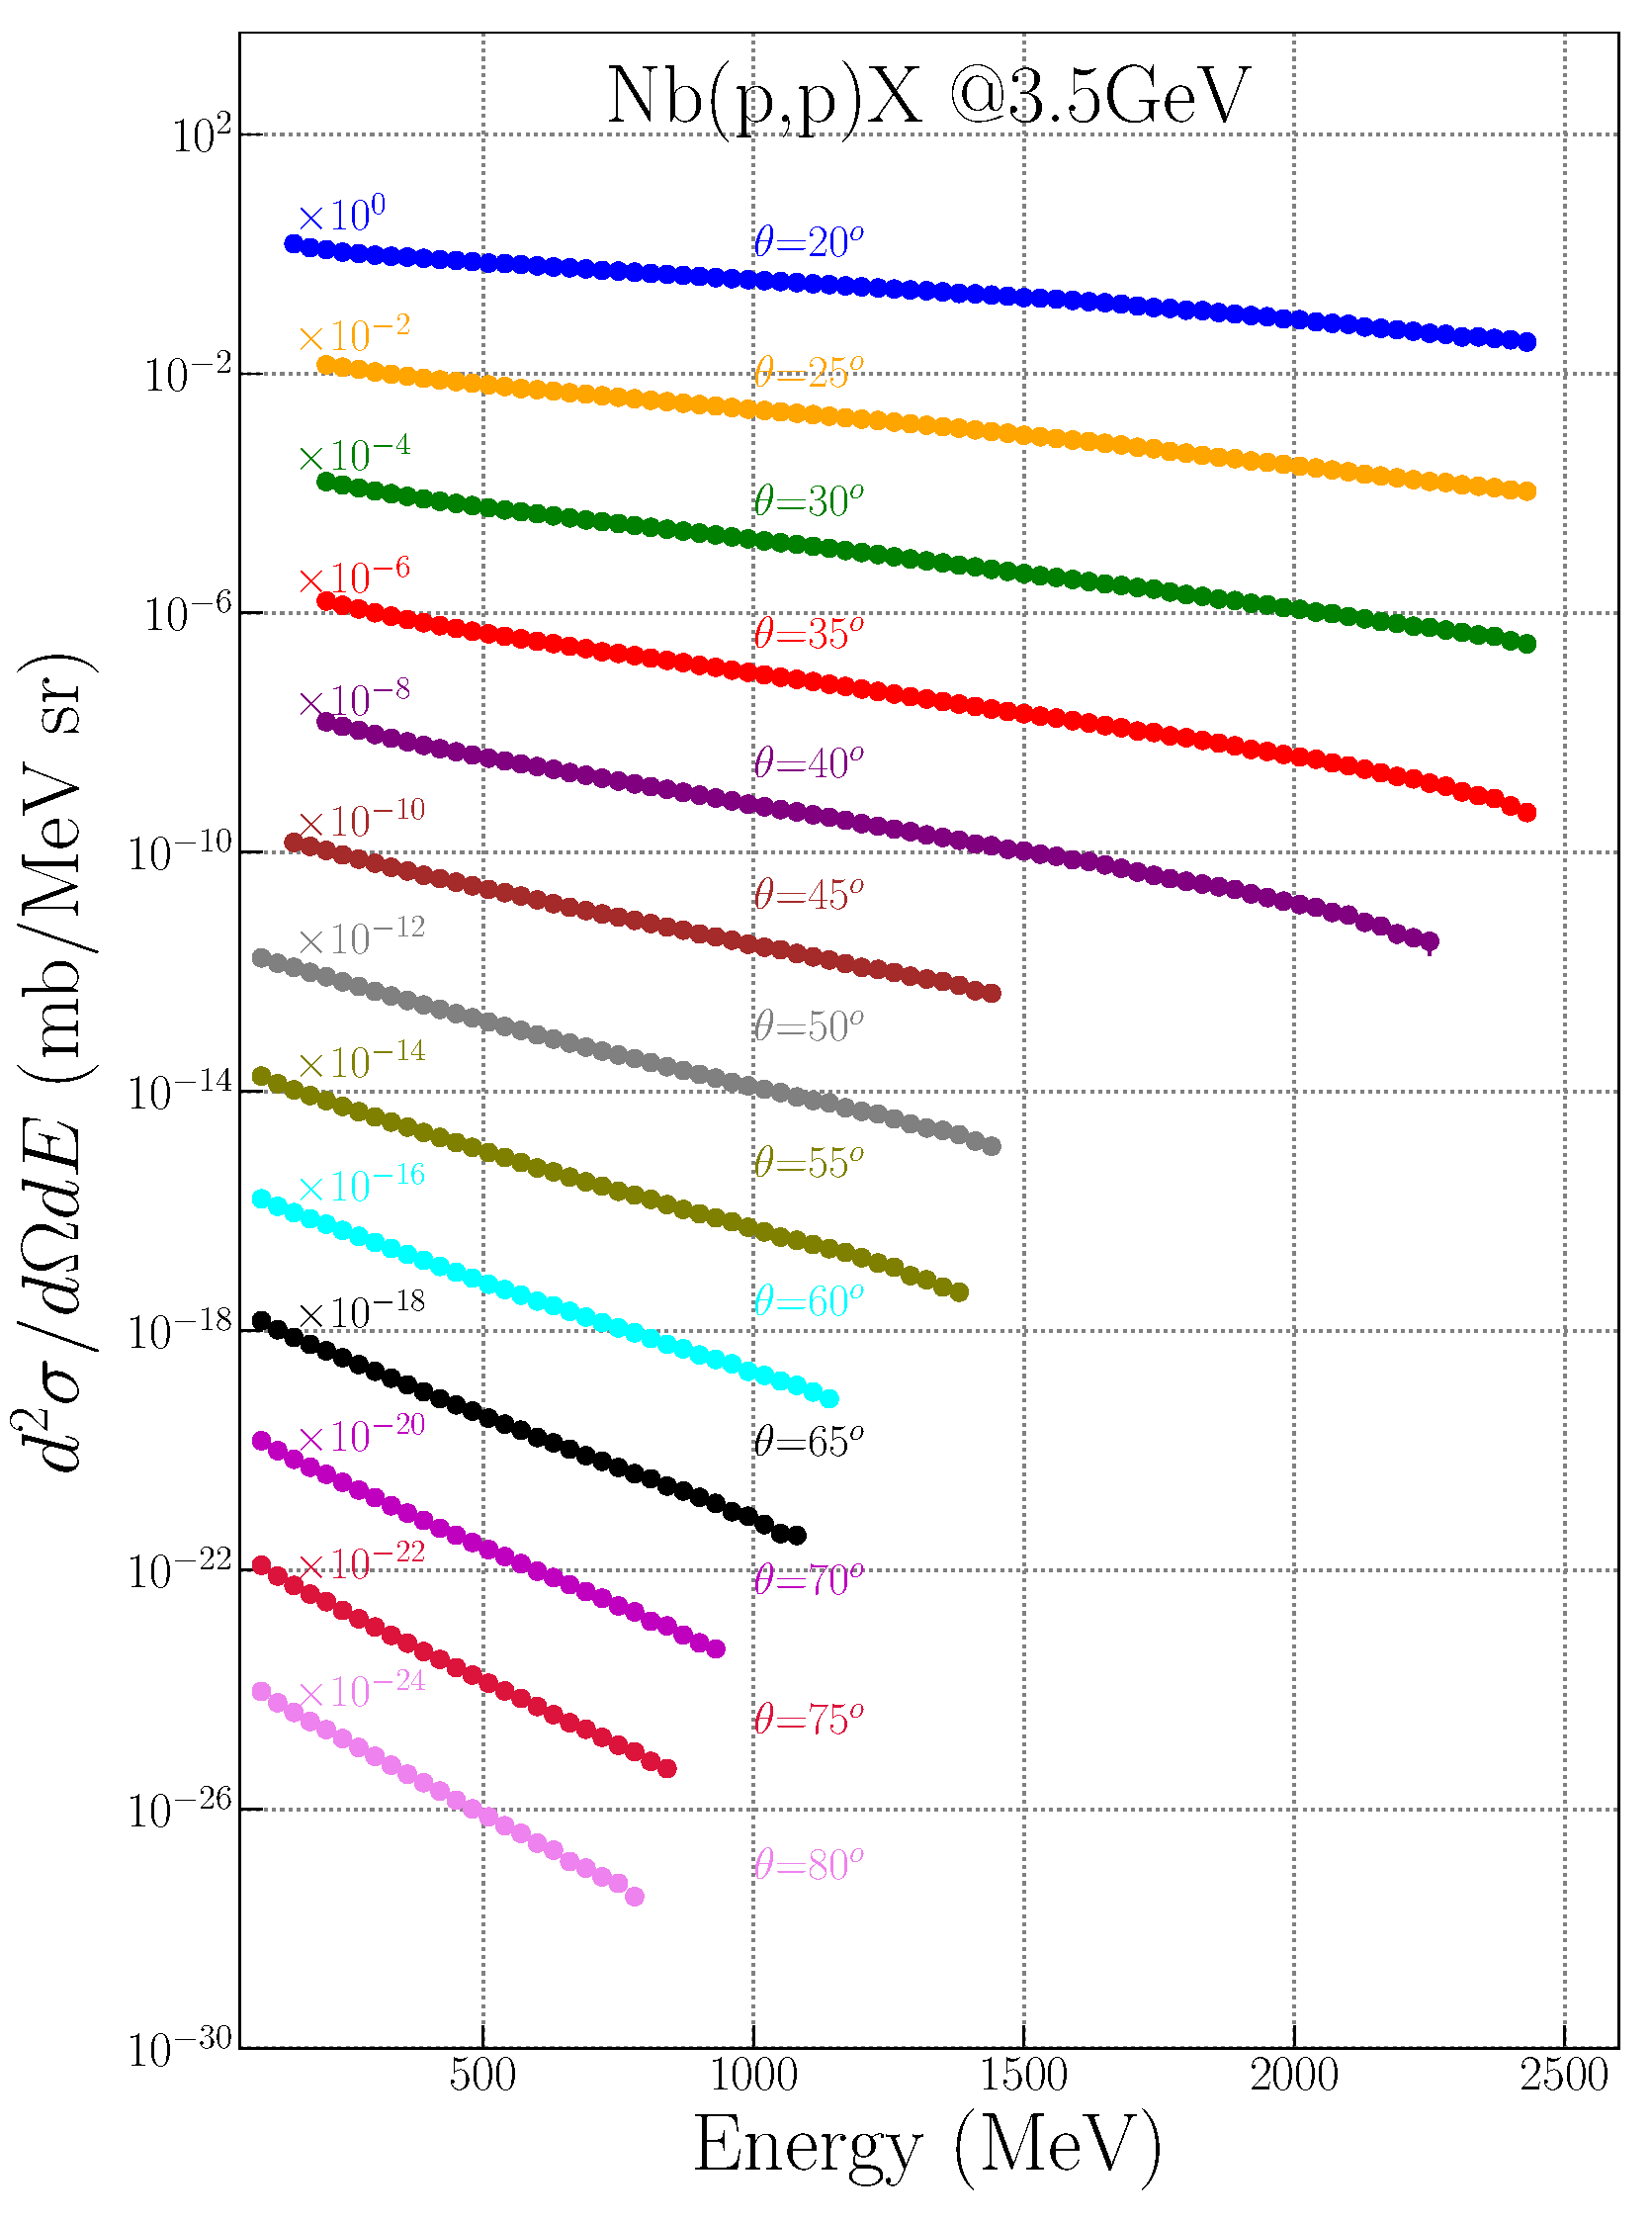
\includegraphics[width=0.67\textwidth] {Protonall.eps}
	\caption{Double differential cross-sections of $p$  measured at HADES 
		in $p$+$^{93}Nb$ reaction at 3.5 GeV incident proton energy (full circles).
		The distributions measured at emission angles of 20$^{\circ}$ $\le$ $\theta$ $\le$ 80$^{\circ}$ with the step of 5$^{\circ}$ are shown.
		In order to facilitate the comparison each distribution at higher angle is multiplied by factor of 10$^{-2}$. }
	\label{Protonall}
\end{figure}
\begin{figure}[!hbt]
\centering
		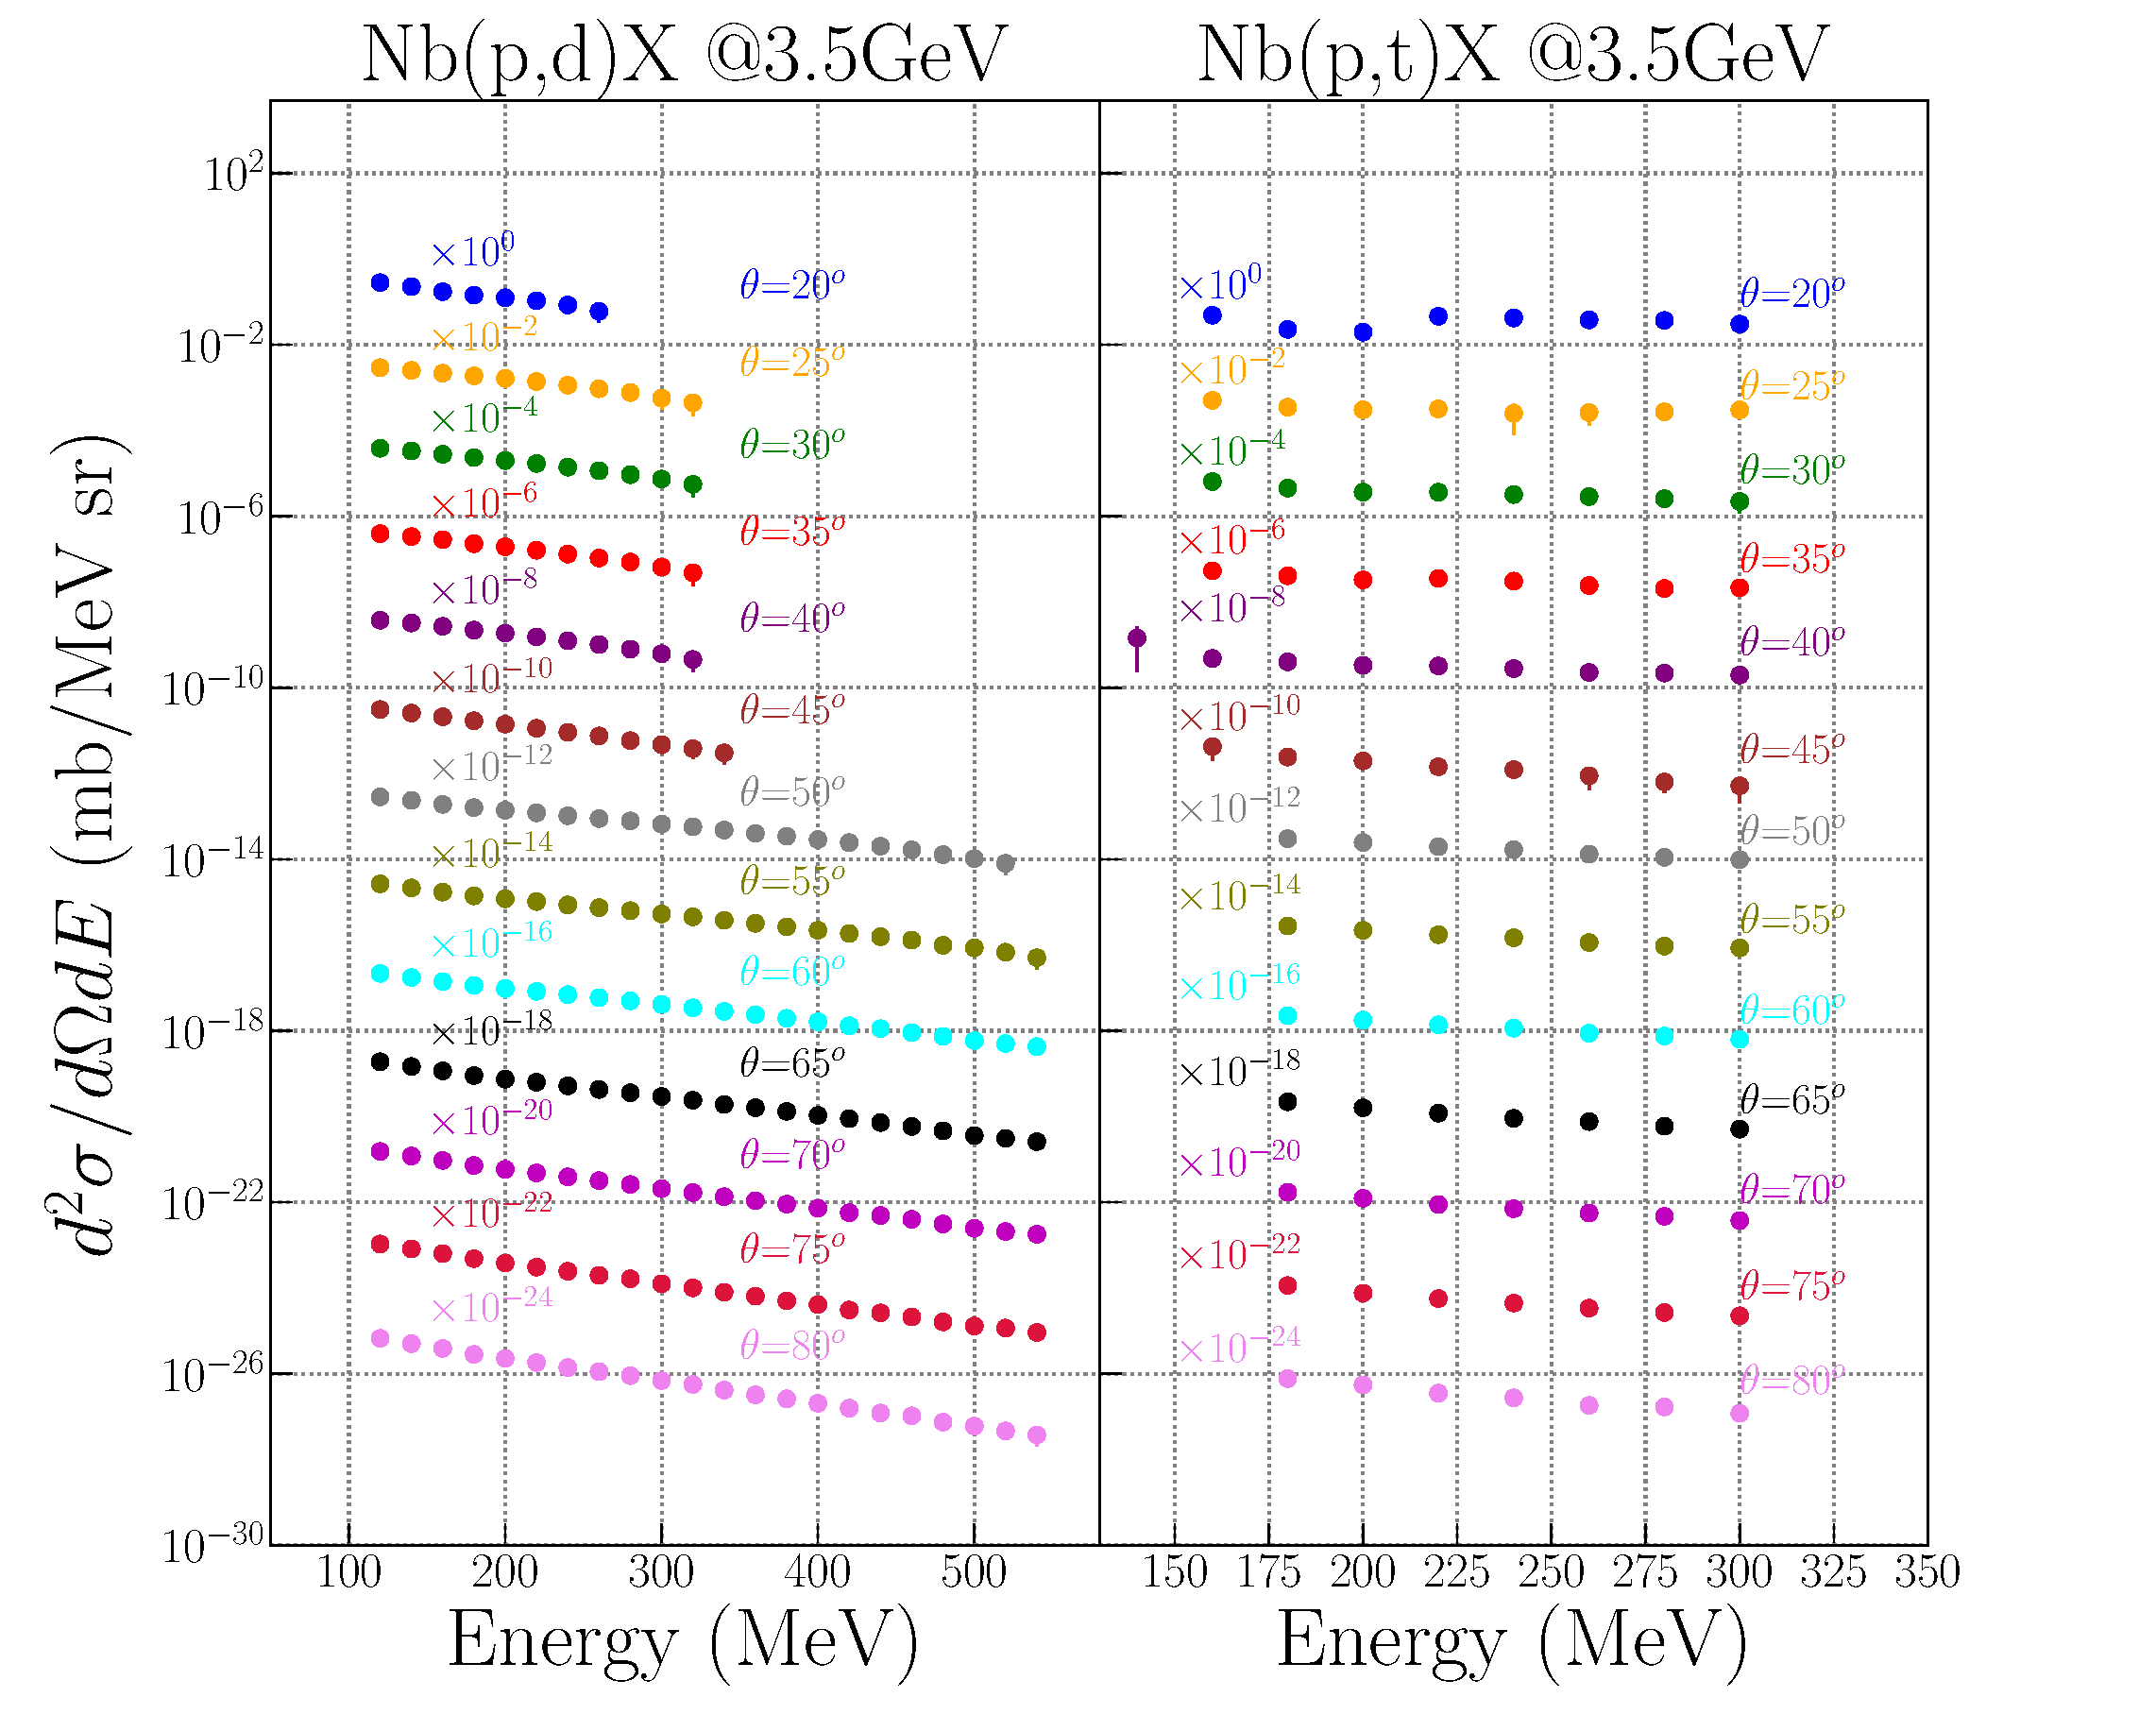
\includegraphics[width=\textwidth] {Deuteronall.eps}
	\caption{\label{pdt_all}
	Double differential cross-sections of $H$ isotopes: $d$ (left panel) and $t$ (right panel) measured at HADES 
		in $p$+$^{93}Nb$ reaction at 3.5 GeV incident proton energy (full circles).
		The distributions measured at emission angles of 20$^{\circ}$ $\le$ $\theta$ $\le$ 80$^{\circ}$ with the step of 5$^{\circ}$ are shown.
		In order to facilitate the comparison each distribution at higher angle is multiplied by factor of 10$^{-2}$.
		% Double differential cross-sections of $p$ measured at HADES in $p+^{93}Nb$ reaction at 3.5 GeV incident proton energy (full circles).
		% The distributions measured at emission angles of 20$^{\circ}$ $\le$ $\theta$ $\le$ 80$^{\circ}$ with the step of 5$^{\circ}$ are shown.
		% In order to facilitate the comparison each distribution of higher angle is multiplied by factor of 10$^{-2}$. 
	}
\end{figure}
% \begin{figure}[!hbt]
% 	\begin{subfigure}[b]{0.49\textwidth}
% 		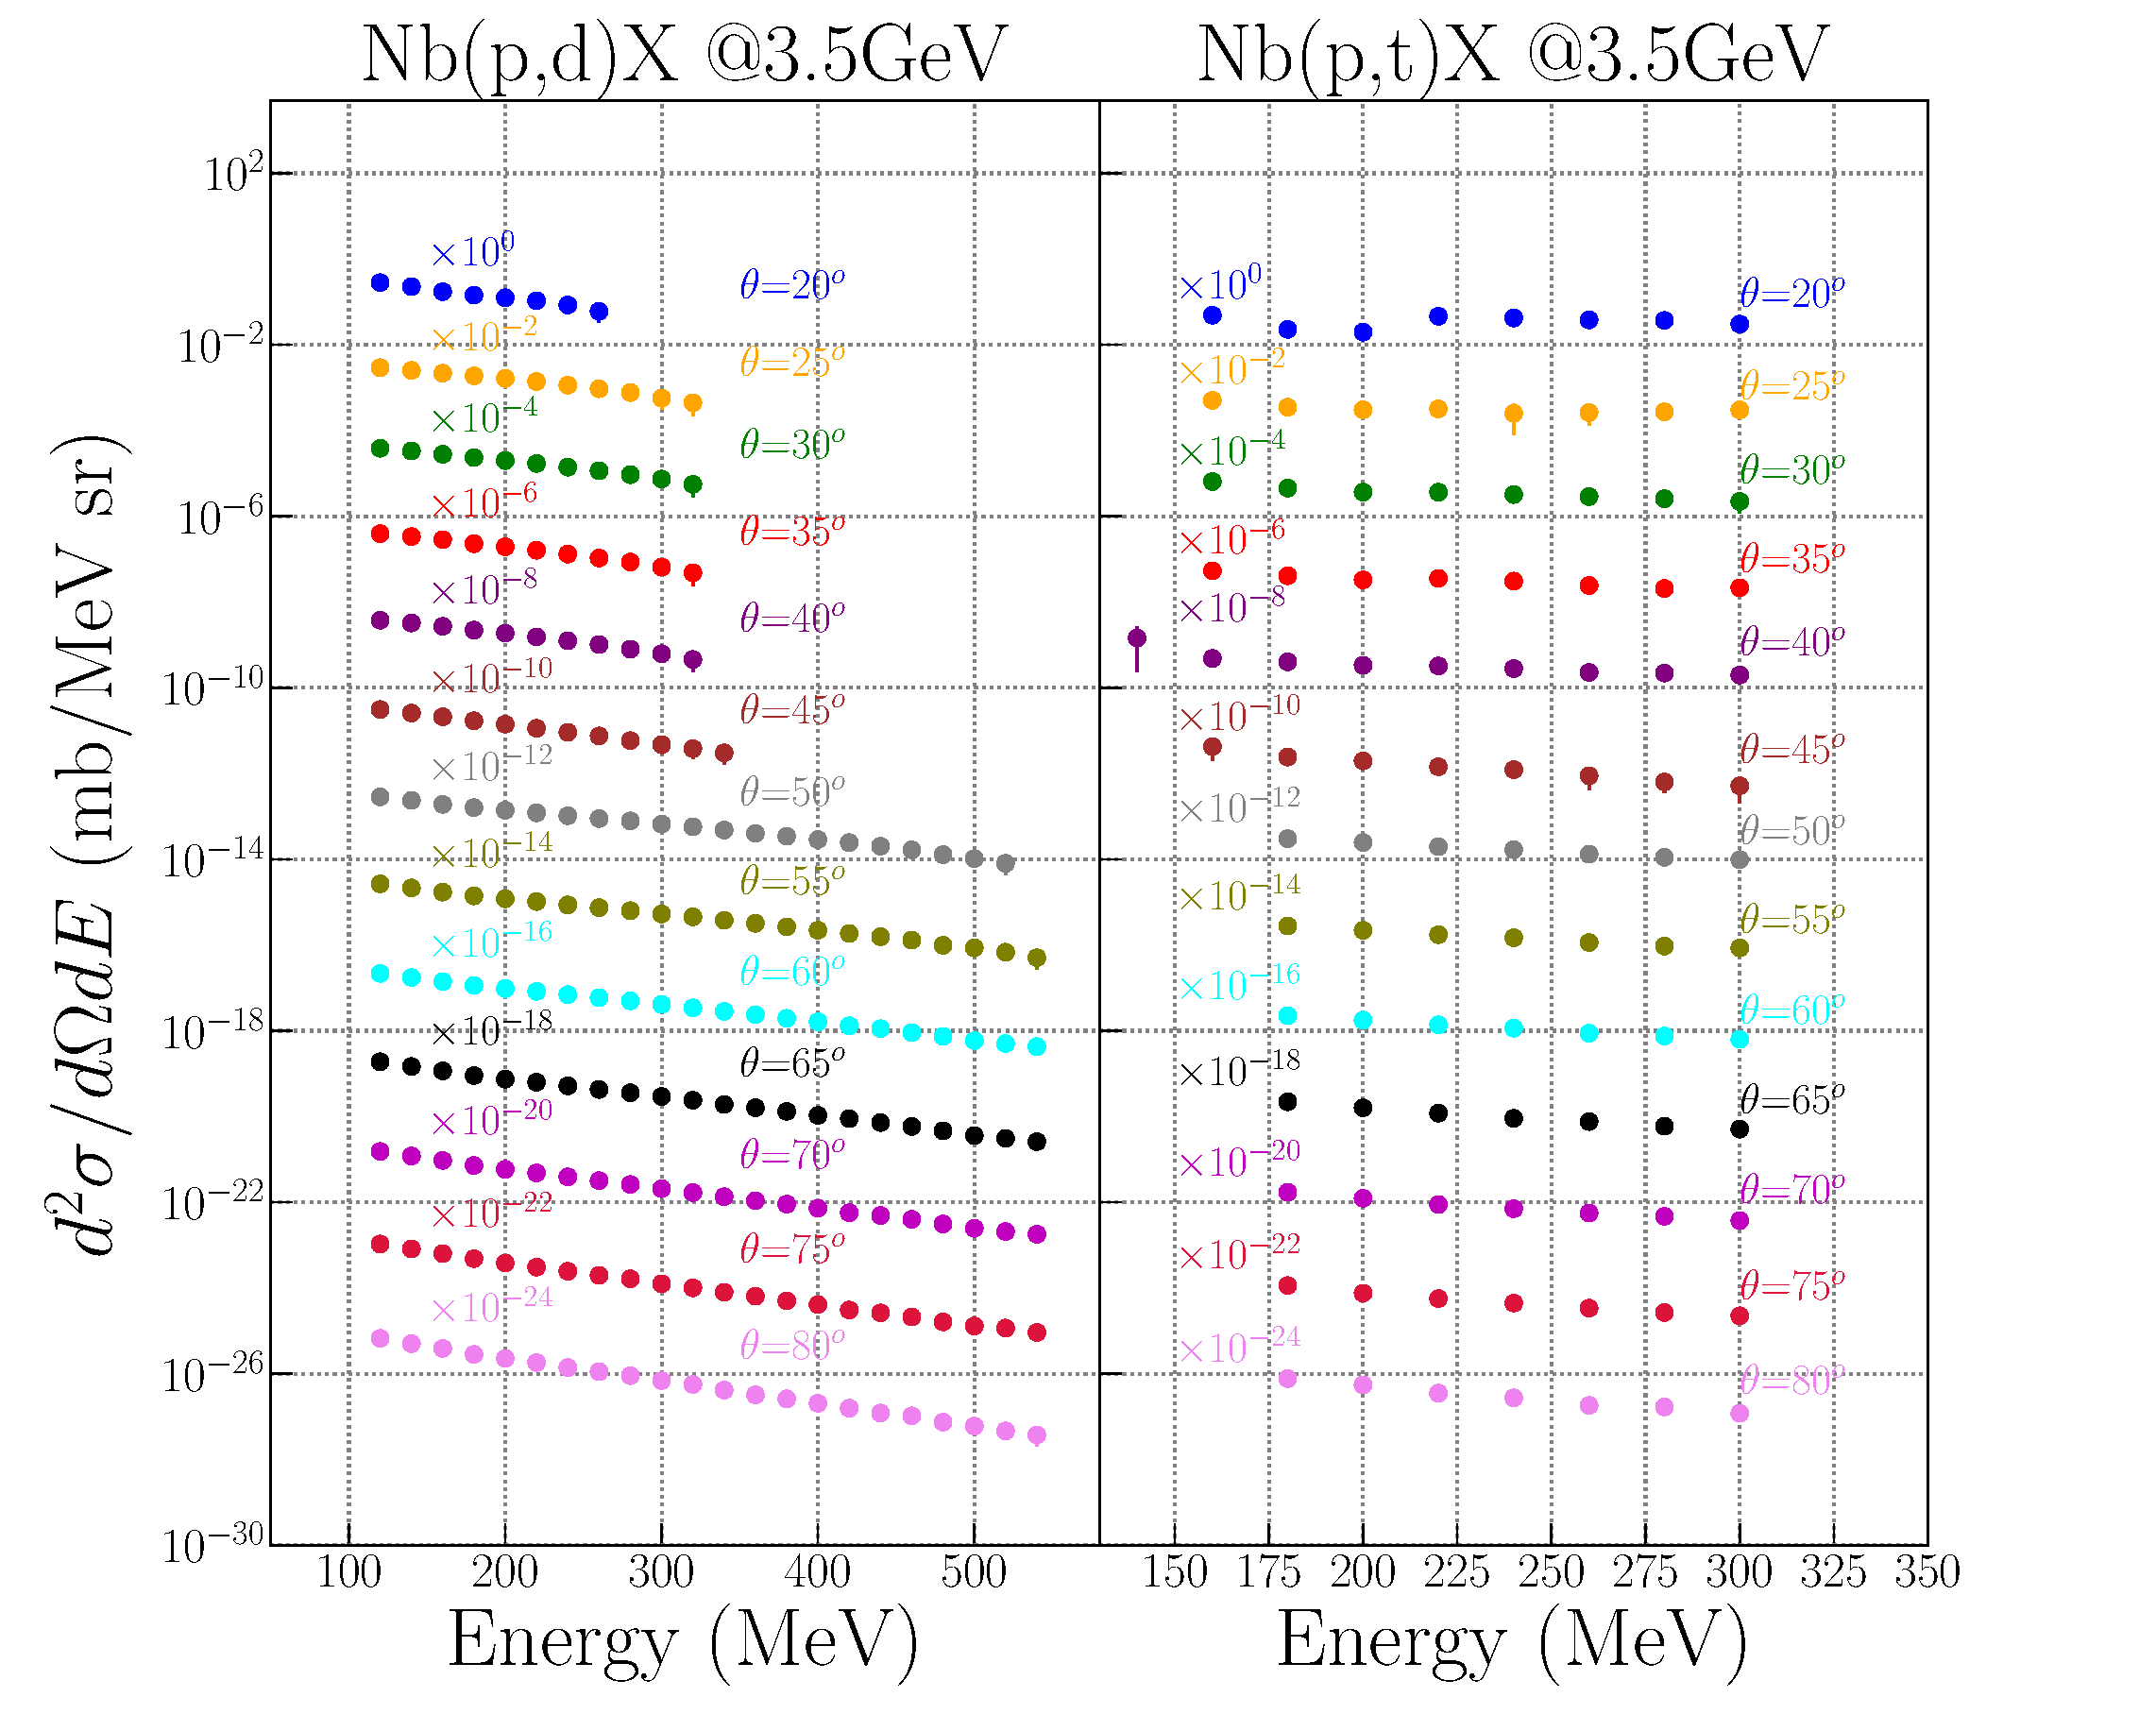
\includegraphics[width=0.9\textwidth] {Deuteronall.eps}
% 		\caption{Deuteron}
% 		\label{Deutronall}
% \end{subfigure}
% 	\begin{subfigure}[b]{0.49\textwidth}
% 	\includegraphics[width=0.9\textwidth] {Tritonall.eps}
% 	\caption{\label{tri_all}triton}	
% 	\end{subfigure}
% 	\caption{\label{pdt_all}
% 		Double differential cross-sections of $H$ isotopes: $d$ (middle panel) and $t$ (right panel) measured at HADES 
% 		in $p+^{93}Nb$ reaction at 3.5 GeV incident proton energy (full circles).
% 		The distributions measured at emission angles of 20$^{\circ}$ $\le$ $\theta$ $\le$ 80$^{\circ}$ with the step of 5$^{\circ}$ are shown.
% 		In order to facilitate the comparison each distribution of higher angle is multiplied by factor of 10$^{-2}$. 
% 	}
% \end{figure}
\begin{figure}[!hbt]
\centering
		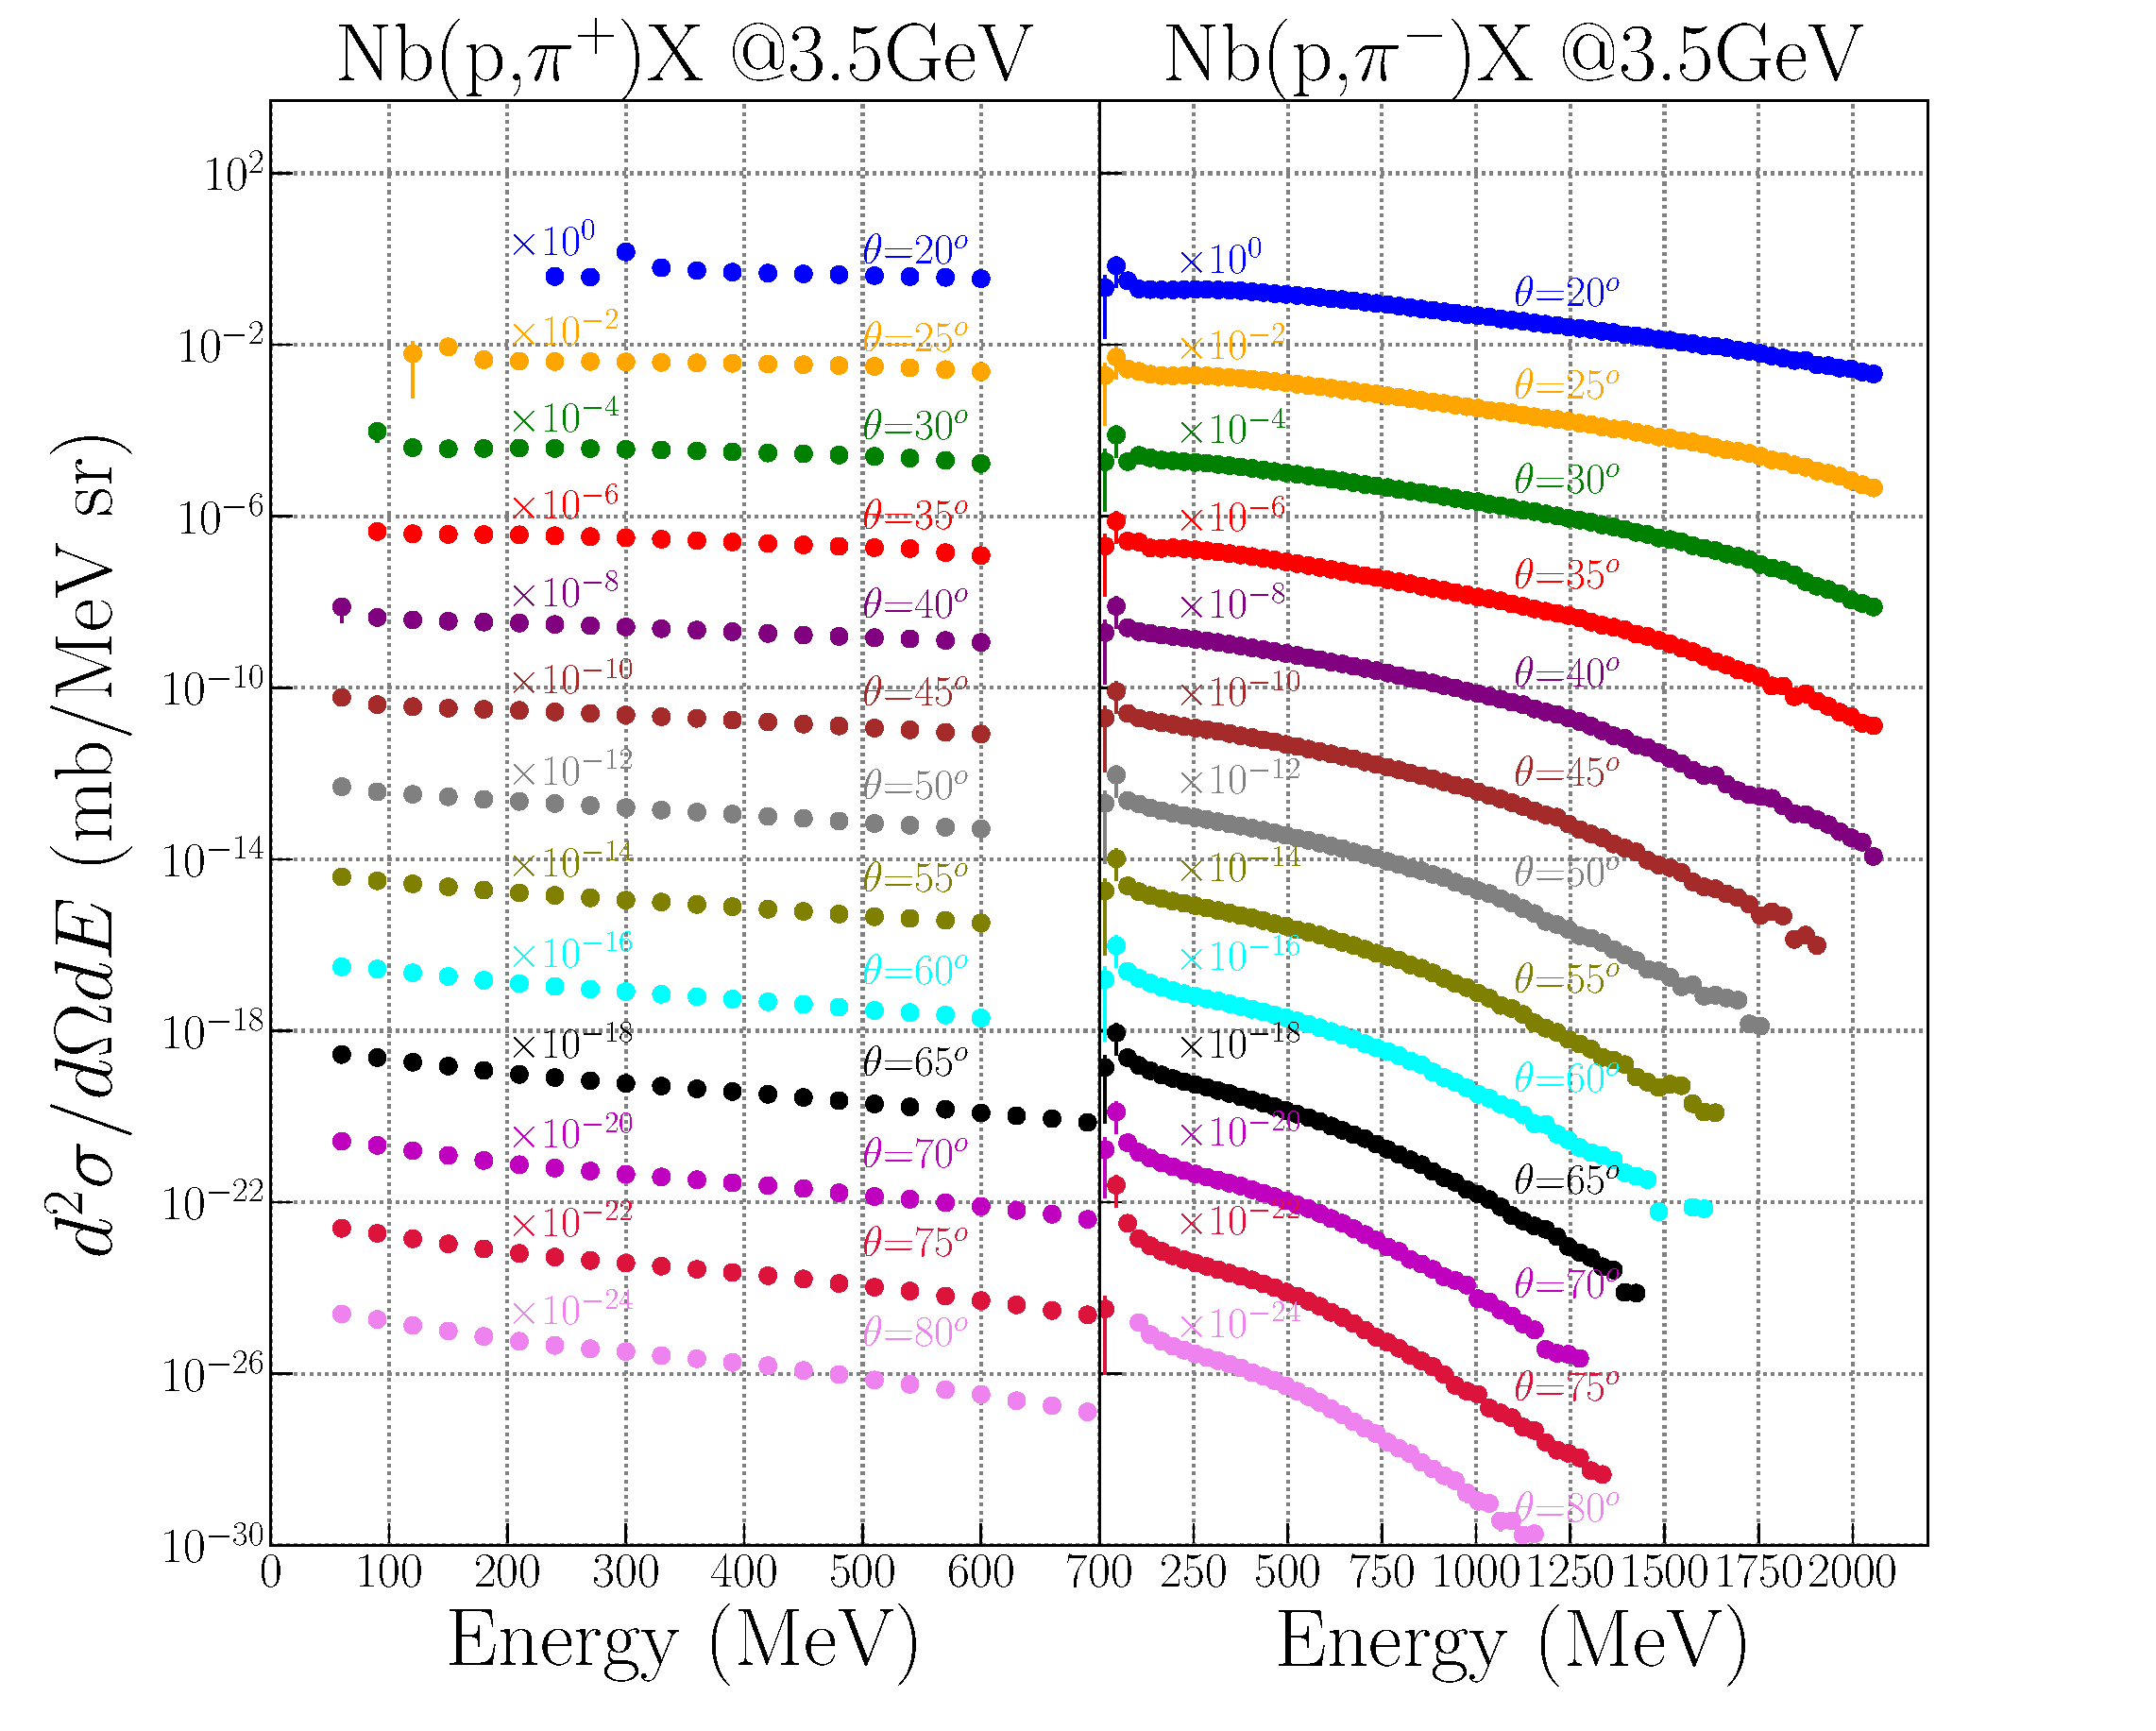
\includegraphics[width=\textwidth] {PionPositiveall.eps}
	\caption{\label{pi_all}
		The same as in fig. \ref{pdt_all} but for $\pi^{+}$ (left panel) and $\pi^{-}$ (right panel).
		% Double differential cross-sections of $p$ measured at HADES in $p+^{93}Nb$ reaction at 3.5 GeV incident proton energy (full circles).
		% The distributions measured at emission angles of 20$^{\circ}$ $\le$ $\theta$ $\le$ 80$^{\circ}$ with the step of 5$^{\circ}$ are shown.
		% In order to facilitate the comparison each distribution of higher angle is multiplied by factor of 10$^{-2}$. 
	}
\end{figure}
% \begin{figure}[!hbt]
% 	\begin{subfigure}[b]{0.49\textwidth}
% 		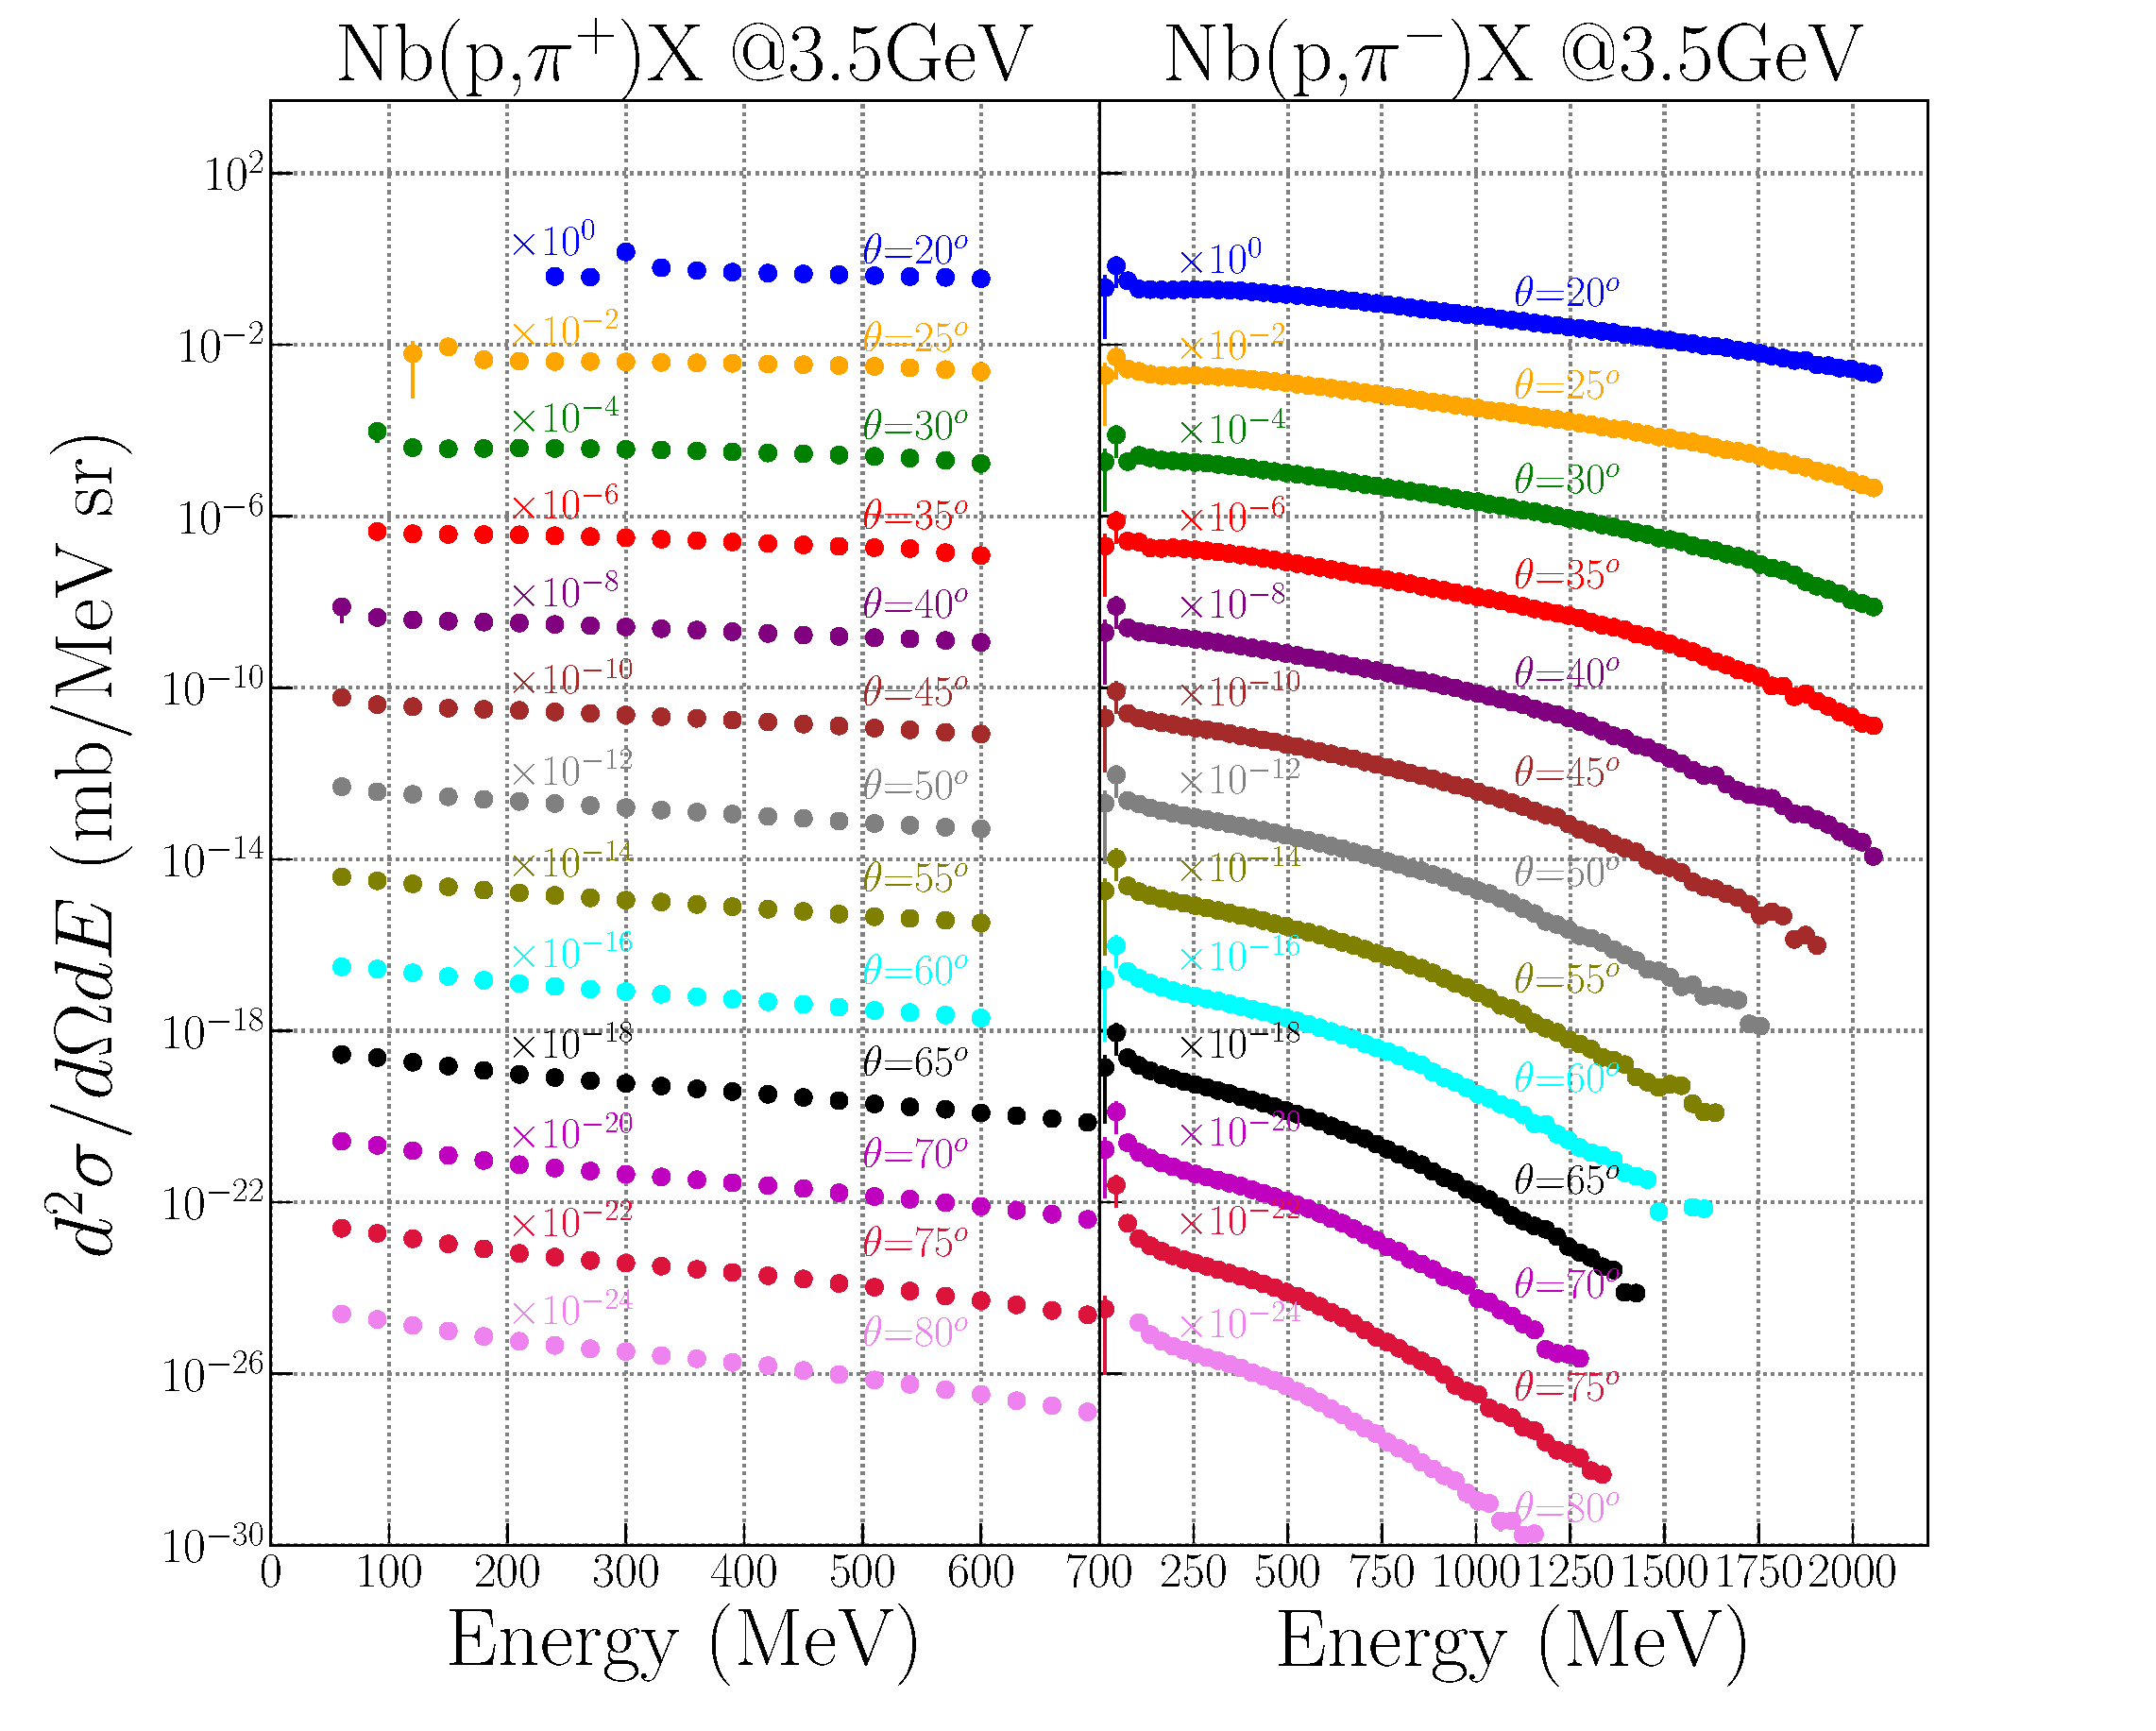
\includegraphics[width=\textwidth] {PionPositiveall.eps}
% 	\end{subfigure}
% 	\begin{subfigure}[b]{0.49\textwidth}
% 		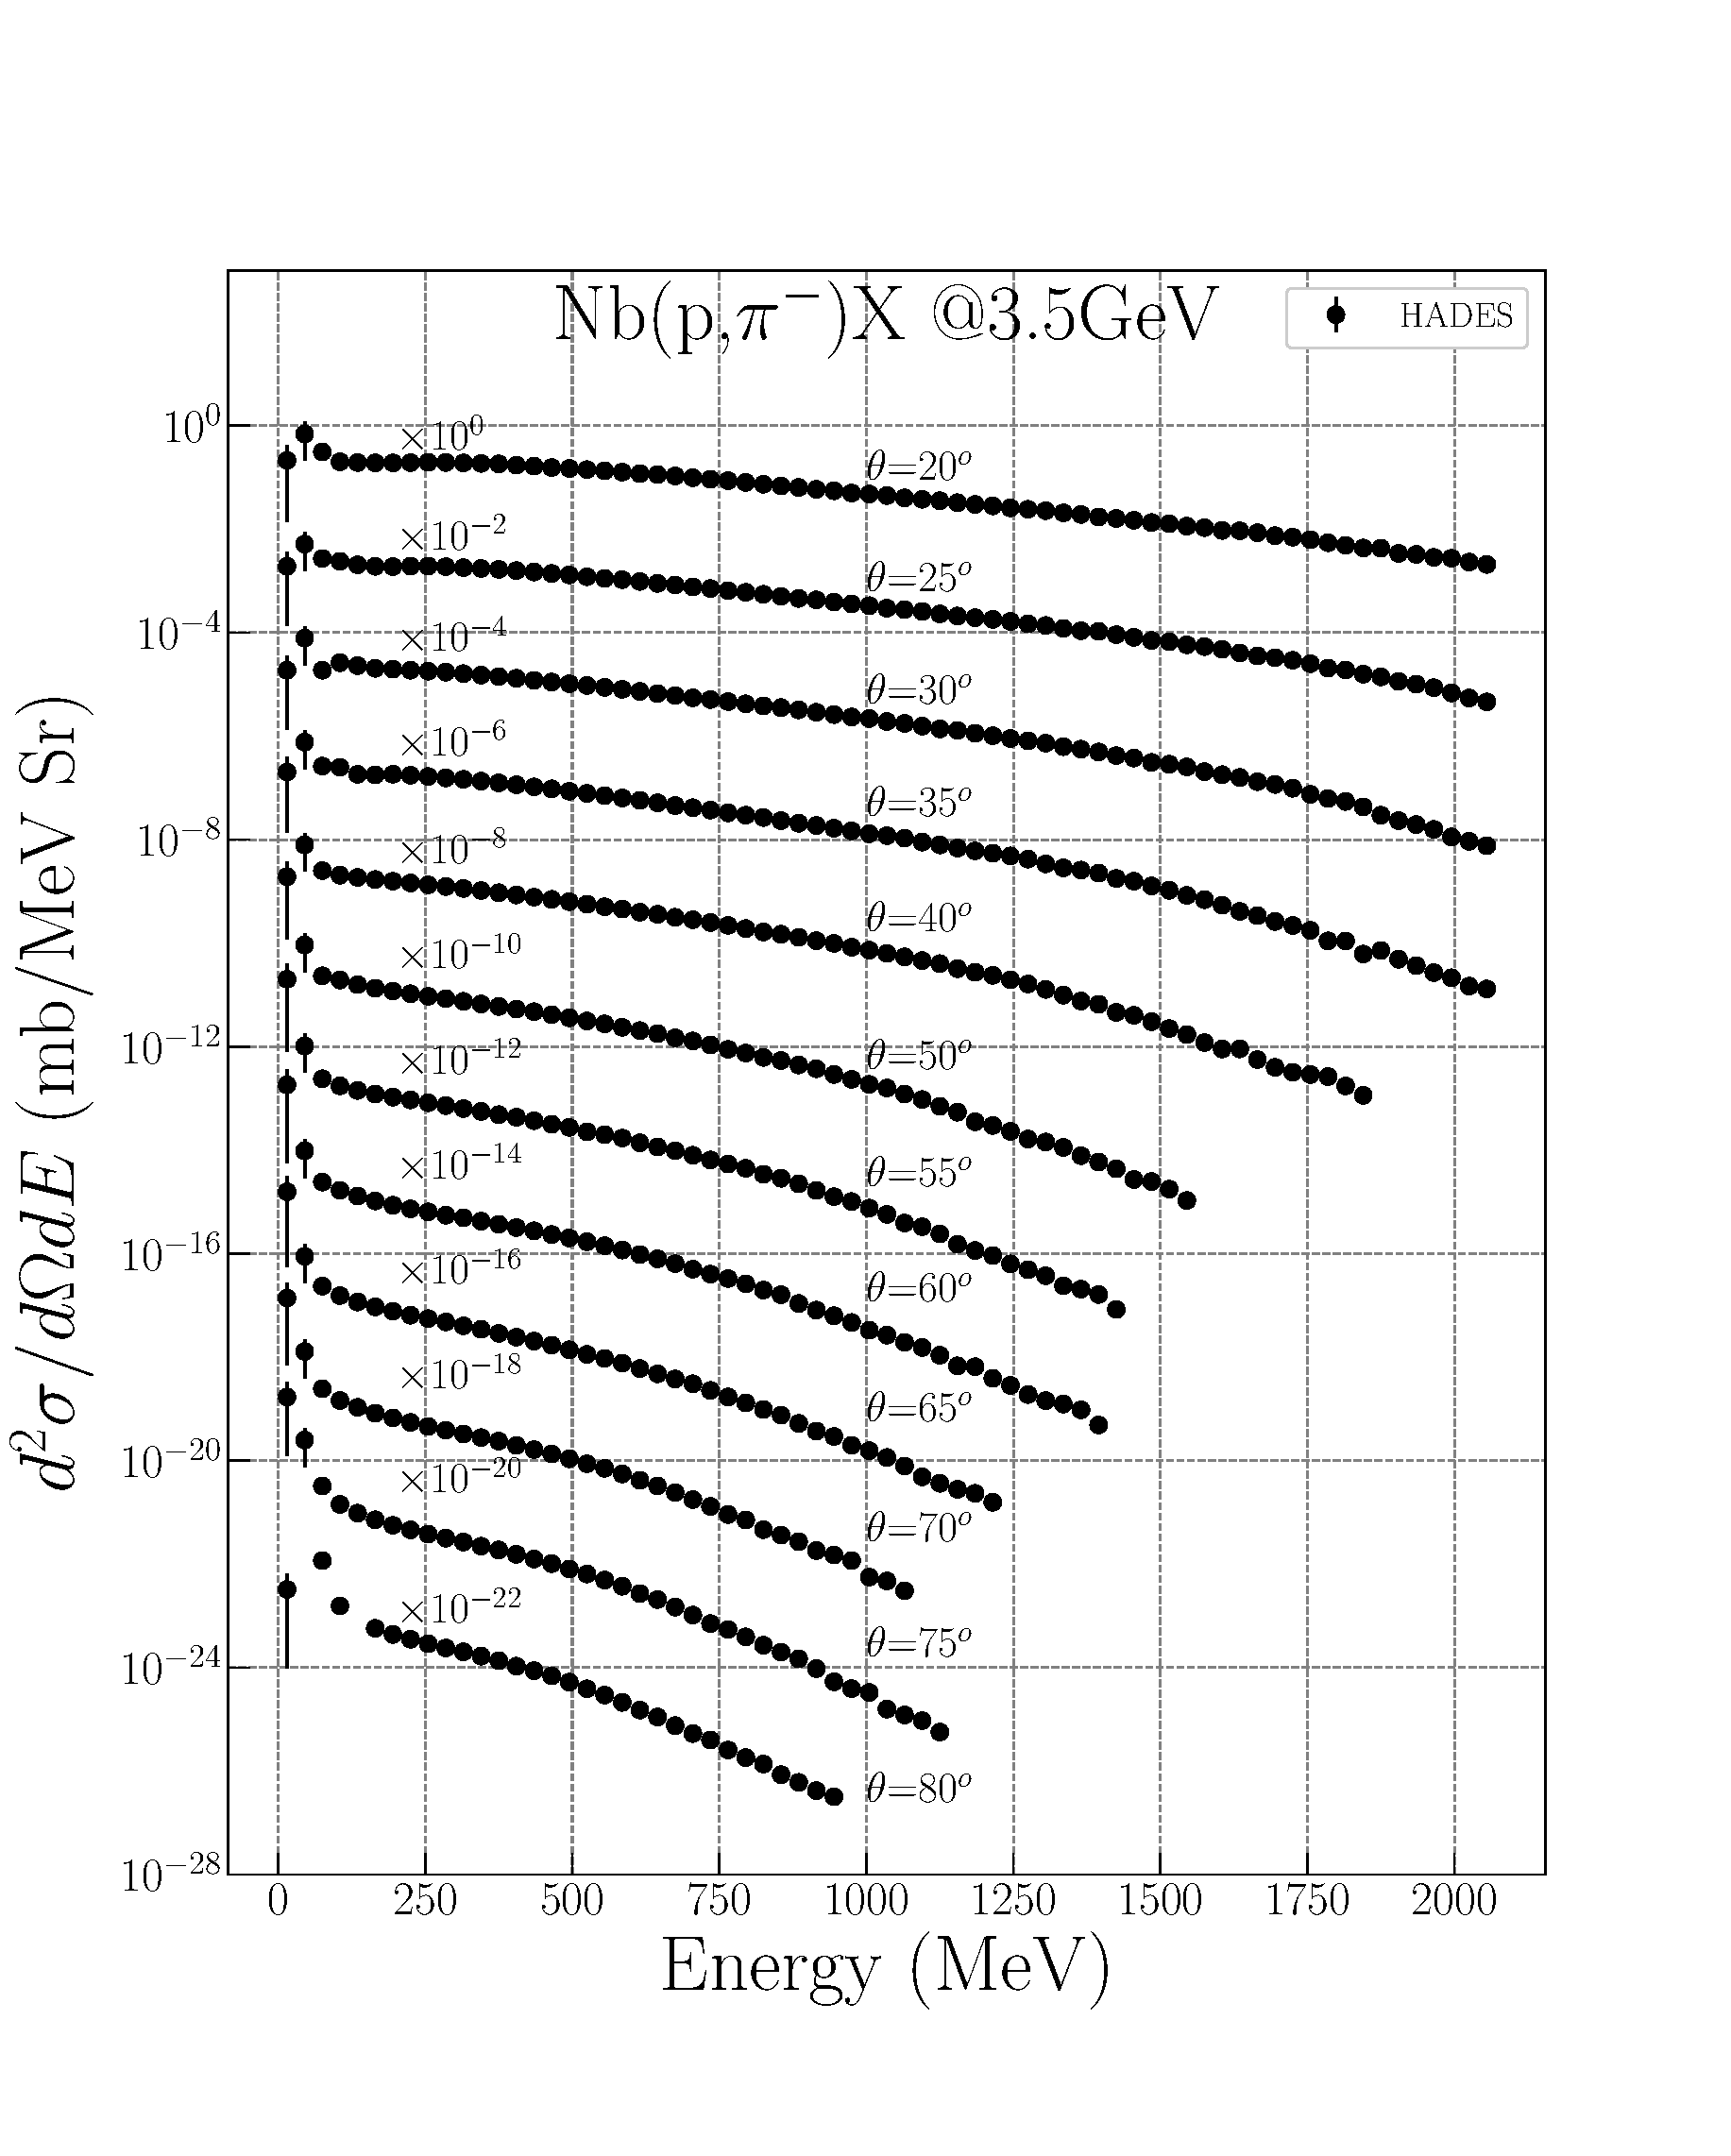
\includegraphics[width=\textwidth] {PionNegativeall.eps}
% 	\end{subfigure}
% 	\caption{\label{pi_all}
% 		The same as in fig. \ref{pdt_all} but for $\pi^{+}$ (left panel) and $\pi^{-}$ (right panel).
% 		% Double differential cross-sections of $p$ measured at HADES in $p+^{93}Nb$ reaction at 3.5 GeV incident proton energy (full circles).
% 		% The distributions measured at emission angles of 20$^{\circ}$ $\le$ $\theta$ $\le$ 80$^{\circ}$ with the step of 5$^{\circ}$ are shown.
% 		% In order to facilitate the comparison each distribution of higher angle is multiplied by factor of 10$^{-2}$. 
% 	}
% \end{figure}

For the aim of current work the $10^8$ events were analyzed. 
Such high statistics of collected and analysed  events permitted to create the $d^2\sigma/d\Omega dE$ distributions for the whole angular range of HADES acceptance, i.e. from 20$^{\circ}$ to 80$^{\circ}$ of the emission angle $\theta$ with the angular step of 5$^{\circ}$. 

The experimental errors are calculated according to formula \ref{Sys_error}, where only the components depending on PID/background error, efficiency + acceptance error and sector error are considered.
%: 
%\begin{equation}
%\label{error}
%\sigma = .....
%\end{equation}
%The total systematic error is calculated as a %square root of sum of squares of uncertainty %components discussed above. 

Such defined uncertainty is calculated for each particle type, selected emission angle $\theta$ and for each energy bin of 30 MeV of the relevant distributions.

The constant component of systematic uncertainty equal to 15\%, resulting from absolute normalisation of HADES data is not included into error bars presented in figures \ref{Protonall}, \ref{pdt_all} and \ref{pi_all}. 
Statistical uncertainties are insignificant and neglected.

In the following the obtained cross-sections are discussed together with their comparison 
to the distributions obtained with the use of three theoretical models. 
Provided here huge set of new and precise experimental data extending to the energies beyond of those available up to now in the literature may put strong 
constraints to each theoretical model which aspires to reasonably
well reproduce mechanism of this stage of the reaction process.



\section{Comparison with the models}
\label{comp_HADES_models}

The processes governing the first stage of proton-target nucleus collision must be reflected in the kinematical distributions of the main reaction products. They are nucleons and pions.
In case of this works particle which carry the information about the proceeding of the intranuclear cascade are protons and charged pions. Moreover, the available single particle 
spectra of the dominant cross-sections are supplemented with the production cross-section of the composite nuclear products, namely the deuterons and tritons. Their rather high energies and forward emission angles indicate that those clusters are created during dynamical phase of the reaction.  

In order to extract the important information
about the process of intranuclear cascade the experimental - angular and energy distributions of charged participants of this process, i.e. protons, pions and complex hydrogen isotopes - deuterons and tritons are compared to the
predictions of the theoretical models. 
They are GiBUU \cite{GiBUUBuss2012}, UrQMD
\cite{UrQMDBleicher1999} and INCL++ \cite{INCLMancusi2014}.
These models are commonly used in investigations
of nucleus-nucleus collisions at GeV/A energies.

As described in chapter \ref{chapter:2} 
the recalled here models differ in the level of approximation of the physical
phenomena appearing in the quantum-mechanical realm of nuclear systems.
They contain some different physics ingredients, and use specific solutions, but in fact they all assume that the intranuclear cascade is a  sequence of binary interactions among the involved nucleons and pions.   

It has to be stressed here that INCL++ model foresees the mechanism for light composite particle production (surface coalescence - cf. chapter \ref{coalesence} and \cite{INCLboudard2013new}) whereas 
both GiBUU and UrQMD are not equipped with the mechanisms allowing for creation of nuclear clusters.

The most up to date versions of the models were used. It was release 2021 (Feb 8, 2021) of GiBUU,
V3.4 for UrQMD and version v6.29-9198542 of INCL++. Also the default settings of each respective model were assumed during all numerical calculations performed in the present study.

\subsection{\label{p_and_pi} Protons and pions}

The main charged reaction carriers inside the struck target nucleus available for the analysis in this thesis are the protons and charged pions.

In order to facilitate comparison of their experimental distributions with the theoretical ones their angular and energy distributions of
cross-sections are given in this subsection 
for only three detection angles of $\theta$ = 25$^{\circ}$, 55$^{\circ}$ and 80$^{\circ}$.
It is justified by the fact that the angular dependence of the data is monotonic and smooth. 

The uncertainties indicated for all presented here experimental data 
include only the energy and angle dependent components of systematic
error - similarly as it was done for complete sets of the HADES results shown above in the section  \ref{comp_HADES_models} (cf. as well the section \ref{Uncertainties}). The absolute normalization uncertainty which is constant an equals to 15\% is not included to the plots. 
The insignificant statistical errors are neglected.

\subsubsection{\label{prot} Protons}

The advantage of the magnetic spectrometer HADES has been fully utilized for selecting the protons emitted from the $p$+$Nb$ reaction. Achieved here range of their measured momenta extends to much higher values than it was possible in earlier experiments dedicated to measurement of production cross-sections of light nuclear products.   

Also their identification suffered the least among all reaction products from the limitation of the identification method based on measuring of the specific energy losses of particles in the detector medium.

In effect the energy range of the cross-sections presented in this work significantly exceeds the energy limits of proton distributions available in the literature.

Obtained distributions are shown in fig. \ref{p_m_3a}. They vary monotonically in the whole detected energy range and their slopes
increase with the emission angle $\theta$. 

The experimental errors are small.
For the logarithmic scale used at the plots mostly they are hidden within the size of the markers.

\begin{figure}[!hbt]
	\centering
	%\includegraphics[width=0.5\textwidth] {/home/pysz/Hades/pNb/Publ/Fig4/Proton.eps}%
	\includegraphics[width=0.8\textwidth] {Proton.eps}%
	\caption{\label{p_m_3a} Double differential cross-sections of $p$
		measured at HADES in $p$+$^{93}Nb$ reaction at 3.5 GeV incident proton
		energy (full circles). Cross-sections are shown for three laboratory
		emission angles of $\theta$=25$^{\circ}$, $\theta$=55$^{\circ}$
		(multiplied by factor 10$^{-1}$) and $\theta$=80$^{\circ}$
		(multiplied by factor 10$^{-2}$). The experimental distributions are
		compared to the results of theoretical models: GiBUU (dash-dotted
		lines), UrQMD (dotted lines) and INCL++ (dashed lines). Constant
		normalization error of experimental data equal to 15\% is not
		included. }
\end{figure}

For the forward emission angles all three models 
provide the proton distributions of the shape which is similar to the experimental ones. But 
the best agreement with the data is provided by GiBUU model. The theoretical curve follow the data at 25$^{\circ}$ in the whole presented energy range. The UrQMD and INCL++ model
underestimate the magnitude of the data by factor larger than 2.
The disagreement of the UrQMD and INCL++ models with the cross-sections measured for protons 
is largest for highest available energies and
decreases with decrease of the kinetic energy of emitted proton. 

The GiBUU starts to overestimate the data   
when the emission angle increases.
But predictions of UrQMD and INCL++ get closer 
to the experimental distribution for larger  angles.

For the largest presented here emission angle of 80$^{\circ}$ the best description of the proton data is provided by INCL++. 
The worst agreement is observed for GiBUU model. It overestimates the experimental cross-section and the discrepancy increases with the proton energy. Disagreement of factor of $\sim$2 is attained at the end of available data range.

\subsubsection{\label{charged_pi} Charged pions}

The experimental energy spectra for
charged pions are shown in fig. \ref{pip_m_3a} (for $\pi^{+}$) and in fig. \ref{pim_m_3a} (for $\pi^{-}$). 

\begin{figure}[!hbt]
	\centering
	%\includegraphics[width=0.5\textwidth] {/home/pysz/Hades/pNb/Publ/Fig4/PionPositive.eps}%
	\includegraphics[width=0.9\textwidth] {PionPositive.eps}%
	\caption{\label{pip_m_3a} The same as in fig. \ref{p_m_3a} but for
		$\pi^{+}$.
		% Double differential cross-sections of $\p$ measured at HADES in $p+^{93}Nb$ reaction at 3.5 GeV incident proton energy (full circles).
		% The experimental distributions are compared to the results of theoretical models: GiBUU (dash-dotted lines), UrQMD (continues lines) and INCL++ (dashed lines).
	}
\end{figure}

In general their energy ranges are broader than those provided up to now in
experiments performing similar research. 
The exception is observed for the forward detection angles of $\pi^{+}$.
In the present analysis - due to limitation of particle identification (PID) based on $dE/dx$ measurement - these particles can't be effectively identified among other reaction products when their energies exceed $\sim$600 MeV.

At most forward emission angles of $\pi^{+}$ (see fig. \ref{pip_m_3a}) the theoretical distributions of all three models underestimate the experimental cross-sections.
It is most significant for lowest energy. Discrepancies decrease when energy of pions increase. For energies greater than $\sim$500 MeV,  results of INCL++ almost follow the data.

The agreement improves with increase of emission angle. All three models follow approximately the shape of experimental spectrum. Theoretical distributions are closest to the data in the range of 250 - 500 MeV of pion energies. 
In general, for the the mid-angular range of HADES, the models agree with the data within the limit of factor 2.

For the highest detection angles of HADES 
almost ideal description of experimental cross-sections for $\pi^{+}$ is provided by UrQMD  model. The most pronounced disagreement is visible for results of INCL++ when the energies of pions are greater than $\sim$500 MeV.

\begin{figure}[!hbt]
	\centering
	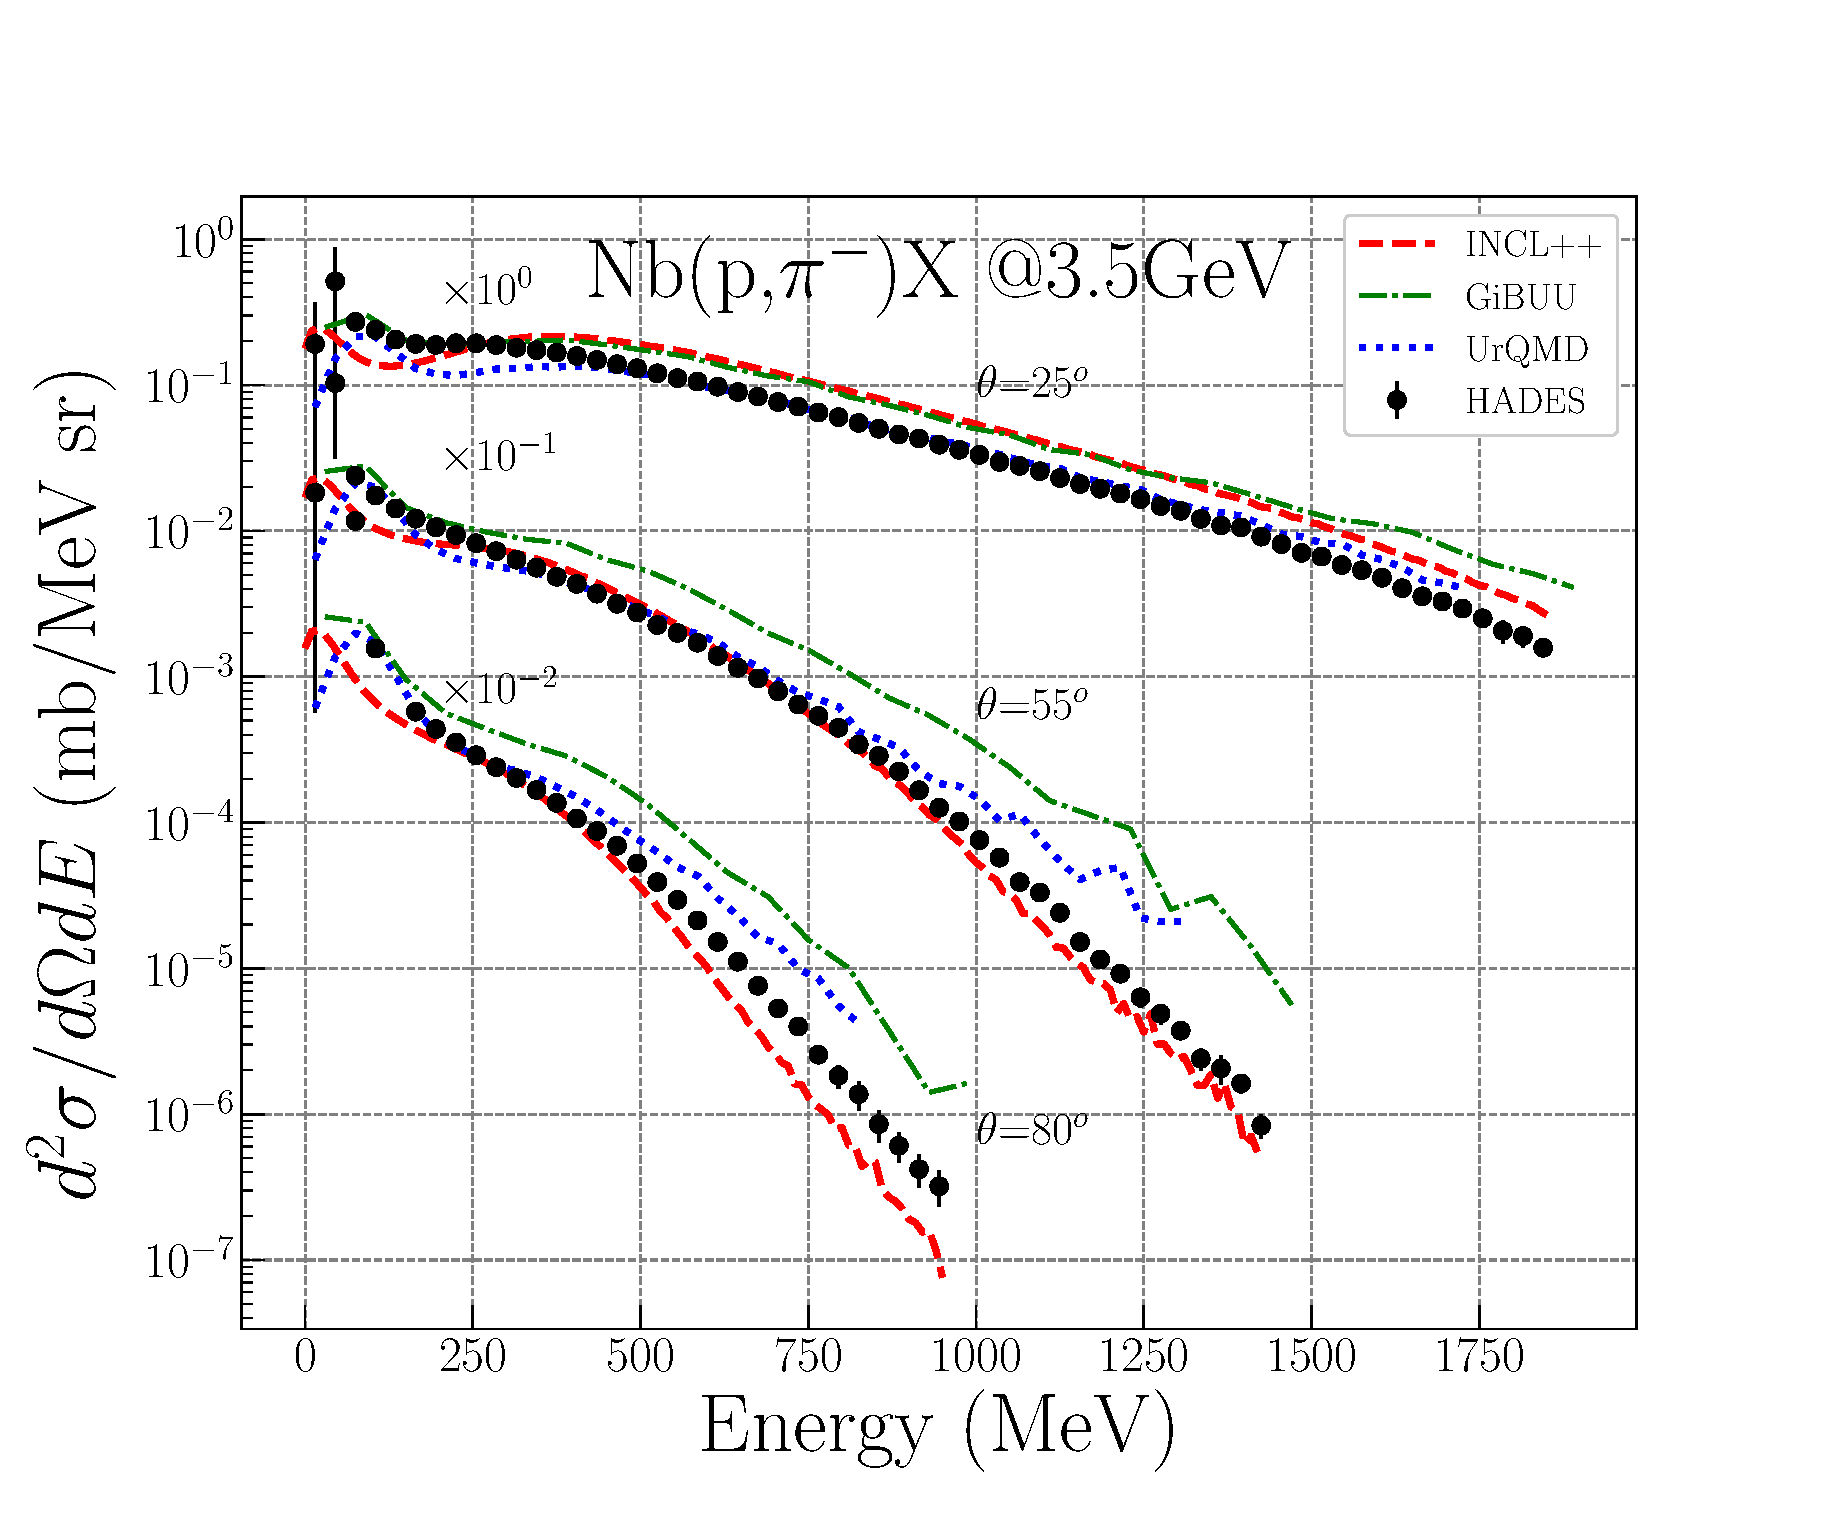
\includegraphics[width=0.9\textwidth] {PionNegative.eps}%
	\caption{\label{pim_m_3a} The same as in fig. \ref{p_m_3a} but for
		$\pi^{-}$.
		% Double differential cross-sections of $\p$ measured at HADES in $p+^{93}Nb$ reaction at 3.5 GeV incident proton energy (full circles).
		% The experimental distributions are compared to the results of theoretical models: GiBUU (dash-dotted lines), UrQMD (continues lines) and INCL++ (dashed lines).
	}
\end{figure}

%\subsection{$\pi^{-}$}

From inspection of fig. \ref{pim_m_3a} it can be concluded that the best description of differential production cross-section for $\pi^{-}$ 
is provided by UrQMD model.

It is especially visible at most forward emission  $\theta$ angle where the agreement is
nearly ideal for almost whole available energy range. Only at pion energies smaller than $\sim400$ MeV the UrQMD underestimates the pion data. 

INCL++ is also rather successful in reproduction of the experimental $\pi^{-}$ cross-section. But it is observed only at middle and highest emission angles. 
However even there, for the lowest and highest energies of detected pions the agreement with 
the data deteriorates. 

The GiBUU model overestimates the $\pi^{-}$ data for all their emission angles and energies available in the present work. Except the smallest energies the discrepancies are at least of factor 5.

\subsection{\label{composite_part} Composite nuclear particles}

The origin of the light composite particles
studied in this work (deuterons and tritons)
is not understood.
The mechanisms responsible for creation of nuclear clusters during the intranuclear cascade are not known.
Various hypotheses of more or less theoretically justified background are proposed
(see e.g. \cite{LET02A,HODGSON20031,Iwamoto_2008,Wei_2014,PyszClus}). 

In INCL++ model the hypothesis of surface coalescence is applied.
It assumes the coalescent origin of composite particles (at least H and He isotopes) which are created still during the pre-thermalization phase of the $pA$ collision. 

Surface coalescence of INCL++ model permits the  dynamical construction of the stable nuclear clusters of the masses A$\le$8. They can be emitted from the target nucleus according to
the conditions implied by the values of their  binding energies and the height of the Coulomb barrier. 

Unfortunately, among the tested theoretical models both GiBUU as well as UrQMD do
not contain the mechanisms responsible for creation of composite nuclear particles.

The HADES experimental double differential cross-sections for both the deuterons as for the tritons are limited in energy. It is due to overlapping of their $dE/dx$ distributions with other H isotopes at higher particles energy. 
Identification of tritons have been especially challenging issue during current analysis.
Nevertheless the obtained results (fig. \ref{d_t_m} for deutrons and for tritons) show the cross-section energy dependence in broader range than that for other 
deuteron and triton data available up to now. 



%Both in fig. \ref{d_t_m} and in fig. \ref{d_t_m} the HADES results
%are confronted with the predictions of INCL++.



The results of simulations of the deuteron distributions with the use of INCL++ model (cf. fig. \ref{d_t_m} - upper panel) overestimate the experimental data. Such disagreement is most pronounced at large emission angles were surface coalescence overestimates the $d$ data by factor $\sim$3. 

At most forward emission angles available in HADES the disagreement is small for low energies of deuterons. But it increases towards larger energies attaining factor of $\sim$3 at the energies $>$300 MeV. In this way the slope of theoretical curve is more flat than for experimental distribution.

The best description of experimental data the INCL++ model and the surface coalescence mechanism provides at middle angles.
For the $\theta$ = 55$^{\circ}$
discrepancy is of factor $\sim$2.

\begin{figure}[!hbt]
	\centering
% 	\begin{subfigure}[b]{0.49\textwidth}
	\includegraphics[width=0.7\textwidth] {Deuteron.eps}%
% 	\caption{\label{d_t_m} deuteron}
% 	\end{subfigure}
% 	\begin{subfigure}[b]{0.49\textwidth}
% 		\includegraphics[width=\textwidth] {Triton.eps}%
% 		\caption{\label{d_t_m} tritons.
% 		}
% 	\end{subfigure}
	\caption{\label{d_t_m}	%The same in fig. \ref{p_m_3a} but for deuterons.
		Double differential cross-sections of deuterons (upper panel) and triton  (lower panel) measured at HADES in
		$p$+$^{93}Nb$ reaction at 3.5 GeV incident proton energy (full
		circles). Cross-sections are shown for three laboratory emission
		angles of $\theta$=25$^{\circ}$, $\theta$=55$^{\circ}$ (multiplied
		by factor 10$^{-1}$) and $\theta$=80$^{\circ}$ (multiplied by factor
		10$^{-2}$). The experimental distributions are compared to the
		results of theoretical model INCL++ (red dashed lines). Constant
		normalization error of experimental data equal to 15\% is not
		included. }
\end{figure}




%The limitations of the method exploring the $dE/dx$ vs. $momentum$
%dependencies for identification of charged particles have the most
%influenced the quality and the energy range of triton cross
%sections. Nevertheless, similarly as for other H isotopes it was
%possible to obtain distributions, which extend in detection energy
%beyond the existing earlier experimental data.
HADES results for $t$ are shown in fig. \ref{d_t_m} - lower panel. Astonishingly the surface coalescence of INCL++ model predicts better the triton
differential production cross-sections than the one for lighter deuterons. The best agreement of experiment and theory is observed tor $t$ emitted at $\theta$ = 55$^{\circ}$. The theoretical curve
agrees with the experimental one for the whole range of registered energies. For lower emission angle the
agreement of the model predictions and the data remains quite good but with slight increase 
of absolute values of discrepancies. At highest detection angles available in this analysis the model starts to overestimate the experiment more visibly. For $\theta$ = 80$^{\circ}$ the disagreement reaches a factor $\sim$2. In the whole angular range of HADES the slopes of
experimental and theoretical distributions are in good agreement.


\section{Interpretation of results}

The general comparison of the HADES experimental
cross-sections for hydrogen isotopes and charged pions and the relevant theoretical distributions of three models has been performed in previous section. 

It was found that the shapes of experimental distributions are in most cases reproduced by the models. The absolute values of differences are usually kept within a factor of 2.

Also the expected behaviour of the theoretical distributions like a smooth decrease of the cross-sections with increasing of the scattering angle and the energy of emitted particles is confirmed. 
Unfortunately, in the whole available kinematic range,  no any systematic behaviour of the 
relationships between experiment and theories can  be observed. 

%It is evident that for
%close investigation of the quality of data reproduction by the
%models some additional means have to be involved.

In order to perform more detailed assessment of the abilities of theoretical models to predict the experimental data the quantity called $A$-factor developed in \cite{sharma2017ranking,singh2018predictive} has been applied.

The great advantage of $A$-factor is that its value quantify the deviation between two discreet distributions of the cross-sections by the number between 0 and 1.

The original formula for $A$-factor is as follows:
\begin{equation}
\label{A_factor_1}
%\[
A \equiv \frac{1}{N}   \sum_{i=1}^{N}  \frac{\left |\sigma^{exp}_{i}
- \sigma^{th}_{i}\right |}{\sigma^{exp}_{i} + \sigma^{th}_{i}}
%\]
\end{equation}
where $\sigma^{exp}_{i}$ and $\sigma^{th}_{i}$ are the values of
experimental and theoretical cross-section in $i$-th histogram bin,
respectively, and $N$ is the number of histogram bins.

For the aim of the current analysis, where
theoretical models are benchmarked both in the domain of laboratory emission angle, $\theta$, as well as in their dependence on the kinetic energy, $E$, of particles, the
$A$-factor was calculated for each bin of two dimensional histogram $\theta$ vs. $E$: 

\begin{equation}
\label{A_factor_2}
%\[
A \equiv  \frac{\left |\sigma^{exp}_{i} - \sigma^{th}_{i}\right
|}{\sigma^{exp}_{i} + \sigma^{th}_{i}}
%\]
\end{equation}

Averaging over several bins as it is
done in formula \ref{A_factor_1} is avoided here.

The properties of factor $A$ are as follows:
\begin{itemize}
    \item it takes values between 0 and 1;
    \item for $A$ = 0 the ideal agreement between compared distributions is observed;
    \item for $A$ = 1  one of the compared cross-sections vanishes or its value become infinite;
    \item value of $A$ is asymmetric depending on the sign of differences between distributions;
    \item for the small differences between the compared distributions the mentioned above asymmetry is small;
    \item in such case the value of calculated $A$-factor can be interpreted as the approximate of the half of relative distance between the data and theoretical cross-sections;
    \item when $A=0.1$ the average relative distance between experimental and theoretical cross-sections is close to 20$\%$;
    \item for $A=0.2$ the average deviation of the cross-sections is close to 40$\%$.
\end{itemize}

In the present studies the experimental and theoretical distributions differ usually within the limits of factor 2. But the individual values of measured cross-sections are charged with uncertainty below 20\%. Thus, for this specific analysis, it is reasonable to introduce gradation of quality of predictive power of the models:
\begin{itemize}
    \item for the calculated value of $A$-factor below 0.1 (maximal difference of the distribution $\sim$20\%) the agreement of two examined distributions is called as "good";
    \item when 0.1 $<$ $A$ $<$ 0.2 (maximal difference of the distribution is in the range of $\sim$20\% to $\sim$40\%) the agreement between distributions is called as "moderate";
    \item values of $A$ $>$ 0.2 call for the conclusion that the agreement between the model and the data is not satisfactory.
\end{itemize}

The uncertainty of $A$-factor itself in the current analysis remains below value of 0.1.
This uncertainty is due to the experimental errors of measured HADES cross-sections which 
are usually below 20\%. 

In figure \ref{Afp_pip_pim_2D} the effect of analysis with the use of $A$-factor is presented.
% The predictive power (PP) of three models for 
% emission of protons and charged pions is shown with the use of contour plots.
% The values of $A$ are indicated 
% in their dependence on particle's kinetic energy $E$ and emission angle $\theta$. 
The contour plots of the $A$-factor in the kinetic energy (E) - emission angle ($\theta$) plane are shown 
%in figure \ref{Afp_pip_pim_2D} 
for emission of protons and charged pions.  They were evaluated by means of three models: GiBUU, UrQMD and INCL++.

% Individual plots of fig. \ref{Afp_pip_pim_2D} permit to define the sensitivity regions of examined models for correlations
% between emission angles and kinetic energies
% of main charged reaction carriers.

\begin{figure*}[!hbt]
\centering
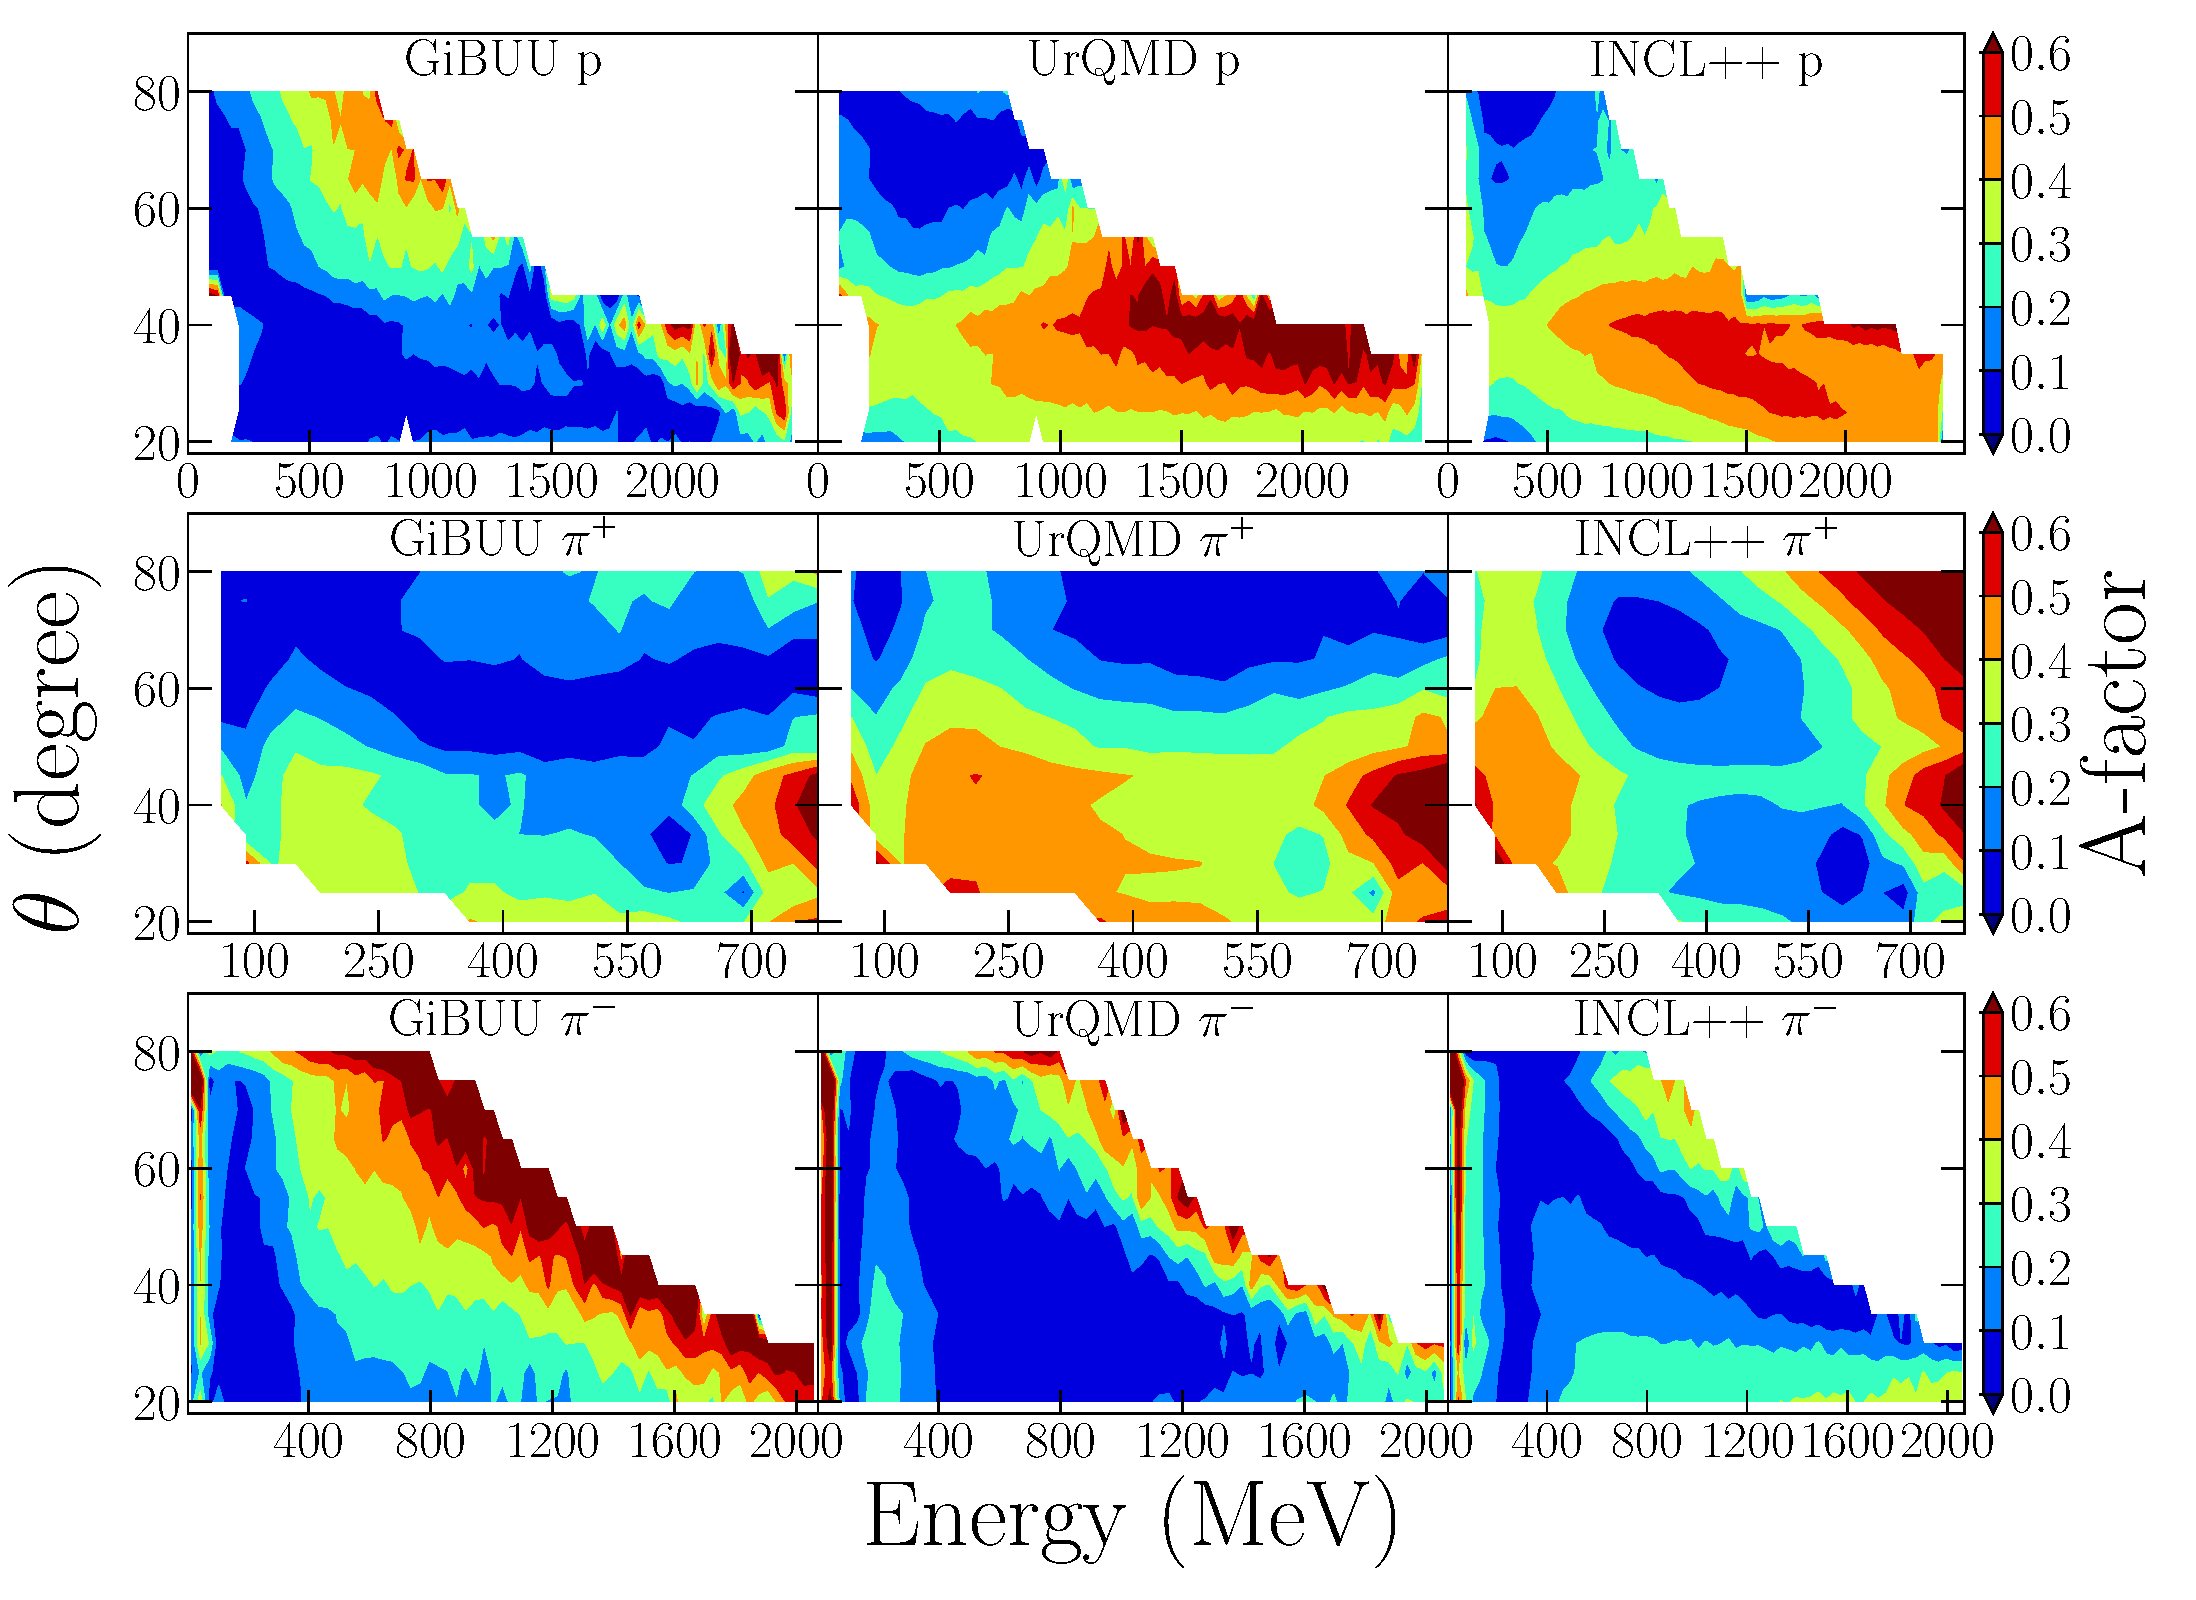
\includegraphics[width=0.97\textwidth]{Afactor2.eps}%
\caption{\label{Afp_pip_pim_2D} Laboratory $\theta$ emission angle
and kinetic energy $E$ dependent distribution of $A$-factor (see text)
for double differential production cross-section of $p$ (upper row),
$\pi^{+}$ (middle row) and $\pi^{-}$ (lower row). It is calculated
according to formula \ref{A_factor_2} for theoretical models of GiBUU (left
column), UrQMD (middle column) and INCL++ (right column) compared to
the experimental values of relevant production cross-section
measured at HADES.
For ideal agreement of the model and the data $A$ = 0 and rises with
the discrepancy between the data and the model. Good and moderate
agreement is observed if $A$ $\le$ 0.2. Note the different energy
scales for the figures in different rows.}
\end{figure*}

%Inspection of the fig. \ref{Afp_pip_pim_2D} confirms to large extend
%the conclusions derived during analysis described in the previous
%section. 

In the most upper three panels of the figure \ref{Afp_pip_pim_2D}
the $A$-factor values of three models for proton data are shown. 
The areas of dark-blue and blue colours corresponding to good 
and moderate agreement between model and
experimental cross-sections are clearly larger for GiBUU than
for two other models. 
It shows that GiBUU is able to provide satisfactory
agreement with the data for significantly larger  
kinematic range of HADES than two other models.  

GiBUU reproduces well the data both, at small and large angles 
and for much broader range of energies for these angles.
However at angles larger than 50$^{\circ}$ it works satisfactory 
at smaller energy range - up to 400 - 500 MeV.
\par
The regions of small values of the $A$-factor of UrQMD and INCL++ corresponds only to angles larger than 50$^{\circ}$ and relatively small energies - smaller than 1000 MeV. 

The middle three panels of fig. \ref{Afp_pip_pim_2D}, 
are devoted to data of positively charged pion and 
their analysis by the same three theoretical models as for protons. 
Inspection of these panels indicate that the regions of angles and energies well described by GiBUU and UrQMD are very similar.  
They cover kinematic range for angles larger than 50$^{\circ}$ (for
GiBUU) and larger than 60$^{\circ}$ (for UrQMD) and for full range of energies (up to 800 MeV). 

INCL++ model describes satisfactorily the data for almost all
angles, however in limited range of energies. 
At angles larger than 50$^{\circ}$ the good and moderate agreement 
with the data is observed  for energies from about 200 MeV to
500 MeV whereas at angles smaller than 40$^{\circ}$ it is a case for energy span from about 300 MeV to 700 MeV.

The lowest three panels of fig. \ref{Afp_pip_pim_2D} show 
the analysis with $A$-factor for negatively charged pions $\pi^{-}$ again simulated with GiBUU, UrQMD and INCL++ models (from the left to the right panel of the figure, respectively). 

It is clear that each of the models describes well  
different kinematic regions of reaction.
In contrast to emission of protons, GiBUU model reproduces smallest part of the data among other models.  
The GiBUU simulations of $\pi^{-}$ distributions reproduce the data 
in the whole angular range of HADES only for small energy range which additionally decreases when the emission angle gets larger. 
At smallest angles of 20$^{\circ}$ - 25$^{\circ}$ this energy interval of good and moderate agreement extends from 100 MeV to 600 - 700 MeV. 
At largest available angles it ranges from about 100 MeV to 250 MeV. 

HADES cross-sections of $\pi^{-}$ in the broadest kinematical range 
are reproduced satisfactory well by UrQMD model.
Areas with $A$ $<$ 0.2 covers full range of the angles whereas 
range of energies decreases with increasing angle. 
For smallest angles the energies of satisfactory agreement extend 
from about 100 MeV to 1700 MeV and at largest angles -  from 100 MeV to about 500 MeV. 

INCL++ describes well and moderately the $\pi^{-}$ data 
at angles larger than 30$^{\circ}$ for broad interval 
of kinetic energies. It extends from 200 MeV to 2000 MeV at 30$^{\circ}$ but decreases when emission angle increases.  
At the largest angle of 80$^{\circ}$ the energy span of satisfactory 
agreement of model and data ranges only from 200 MeV to 650 MeV.

 \par

Conclusions derived from inspection of $A$-factor distributions for 
$p$, $\pi^{+}$ and $\pi^{-}$ obtained for three theoretical models
are in the perfect agreement with those
from the analysis of single distributions of these particles 
where experimental spectra are compared to model predictions at
three angles: 25$^{\circ}$, 55$^{\circ}$ and 80$^{\circ}$ 
(cf. figs. \ref{p_m_3a} and discussion in subsection \ref{p_and_pi}). 
Such an agreement proves reliability of the present method 
of reasoning based on two-dimensional maps of the $A$-factor values.
 
\par
 
Similar analysis of $A$-factor value as a
function of energy and emission angle of the reaction product can be performed also for deuterons and tritons. However, the
data for emission of these particles can be compared only with
predictions of the INCL++ model. As it was informed already in chapter 
\ref{chapter:2} both in GiBUU as in UrQMD models the mechanisms permitting the creation of nuclear clusters during the intranulcear cascade are not implemented.

The maps with $A$-factor dependence on the product energy 
and emission angle for deuterons and tritons produced in 
$p$ + $Nb$ collision at 3.5 GeV in HADES are presented
in fig. \ref{Afd_t_theta_E}.
%\par
\begin{figure*}[!hbt]
\includegraphics[width=0.95\textwidth] {Deuteron_Triton_Afactor_INCL.eps}%
\caption{\label{Afd_t_theta_E} Dependence of $A$-factor (see text)
on the deuteron (left panel) and triton (right panel) emission angle
$\theta$ and kinetic energy $E$. $A$-factor is calculated according
to the formula \ref{A_factor_2} for comparison of experimental double
differential cross-sections of HADES with the results of theoretical
model INCL. For ideal agreement of the model and the data $A$ = 0
and rises with the discrepancy between the data and the model. Good
and moderate agreement is observed if $A$ $\le$ 0.2. }
\end{figure*}
Distribution of the $A$-factor calculated for INCL++ 
%(v6.23) 
predictions for deuterons confronted with the HADES data indicates that good and
moderate agreement is observed for the all energies of $d$ 
but emitted in the narrow angular range from about 50$^{\circ}$ to about 60$^{\circ}$ of $\theta$ laboratory angle.
Besides these regions the satisfactory reproduction of $d$ data 
INCL++ 
%(v6.23) 
provides for the highest energies and emission angles and 
for low energies below 250 MeV but only for emission angles between 
30$^{\circ}$ - 45$^{\circ}$.
 
For tritons good and moderate agreement is
obtained for all angles larger than about 40$^{\circ}$. 
Additionally the predominantly moderate agreement is visible 
for energy smaller than approximately 270 MeV and at angles smaller than 40$^{\circ}$.

 \par

The two dimensional distributions 
of $A$-factor allows for extraction further credible information,
namely the predictive power (PP) of given theoretical model for selected set of observed particles.

This can be obtained by observation how big is the part of studied
kinematic space of energy - emission angle for which the model describes the data in good and moderate manner ($A$-factor values are smaller or equal to 0.2). 
The ratio of number of such bins to number of all observed bins 
is used as numerical measure of the predictive power (PP) of given model for selected set of observed particles.

Table \ref{Table1} contains the appropriate percentages of
such calculated correctness of individual models for selected individual particles and for their particular and total yields.

\begin{table}%[H] add [H] placement to break table across pages
%\begin{center}
\caption{\label{Table1} Measure of predictive power (PP) of GiBUU,
UrQMD and INCL++ models for double differential cross-sections of
$p$, $\pi^{+}$, $\pi^{-}$, $d$ and $t$ measured at HADES. PP is
equal to fraction of area (in [\%]) of the $\theta$ vs. $E$
distributions presented in figs. \ref{Afp_pip_pim_2D} and
\ref{Afd_t_theta_E} where the agreement of the theoretical model and
the experimental specta of HADES is good ($A$ $<$ 0.1) or good and
moderate ($A$ $<$ 0.2). The predictive power for the simulation of
intranucelar cascade is given for the sum of $p$, $\pi^{+}$ and
$\pi^{-}$ ejectiles. The correctness of reproduction of composite
particle production is calculated for the sum of $d$ and $t$ (only
for INCL++). The overall agreement of the INCL++ model with the data
for all detected in HADES particles is given for the sum of them.
The number corresponding to several emitted types of particles were calculated as percentage of "good" bins for given set of particles  among all bins corresponding to this set of particles.
}
\begin{tabular}{| p{2.2cm}|| p{1.4cm} | p{1.4cm} || p{1.4cm} | p{1.4cm} || p{1.4cm} | p{1.4cm}|}
\hline
\bf{Ejectile} & \multicolumn{2}{c}{\bf{GiBUU}}  & \multicolumn{2}{|c} {\bf{UrQMD}} & \multicolumn{2}{|c|} {\bf{INCL++}} \\
\hline 
& $A$ $<$ 0.1 & $A$ $<$ 0.2 & $A$ $<$ 0.1 & $A$ $<$ 0.2 & $A$
$<$ 0.1 & $A$ $<$ 0.2
\\
\hline \hline $p$ & 39\% & 65\% & 13\% & 25\% & 5\% & 19\%
\\
\hline $\pi^{+}$ & 28\% & 58\% & 19\% & 33\% & 27\% & 35\%
\\
\hline $\pi^{-}$ & 12\% & 28\% & 45\% & 68\% & 33\% & 63\%
\\
\hline $d$ & & & & & 18\% & 52\%
\\
\hline $t$ & & & & & 43\% & 76\%
\\
\hline \hline $d+t$ & & & & & 27\% & 60\% 
\\
\hline \hline $p+\pi^{+}+\pi^{-}$ & 26\% & 49\% & 27\% 
& 43\% & 16\% & 39\% 
\\
\hline \hline $p+\pi^{+}+\pi^{-}+d+t$ & & & & & 19\% & 43\% \\
\hline
%Lines of table here ending with \\
\end{tabular}
%\end{center}
\end{table}


From inspection of the table \ref{Table1} the following conclusions
can be derived:
\begin{itemize}
    \item none of the applied theoretical models is able to reproduce "well" (i.e. with $A < 0.1$) at least a half (i.e. 50$\%$) of the full examined in this thesis $E$-$\theta$ space. It is a case both for each individual of observed ejectiles ($p$, $d$, $t$, $\pi^+$, $\pi^-$) as well as for their combinations ($p$ + $\pi^{+}$ + $\pi^{-}$, $d$ + $t$ and  $p$ + $\pi^{+}$ + $\pi^{-}$ + $d$ + $t$);
    \item GiBUU model reproduces with "good and moderate" 
    quality 65\% of $p$, 58\% $\pi^{+}$ but only 28\% of $\pi^{-}$. 
    In average over all these particles such quality of description is reached for 49\% of $E$-$\theta$ area under investigation;
    \item UrQMD and INCL++ models reproduce "well and moderately" 
    the $p$ and $\pi^{+}$ distributions in less than 50$\%$ situations;
    \item $\pi^{-}$ data are reproduced "well and moderately" in more than in 50$\%$ by UrQMD (68\%) and INCL++ (63\%) whereas GiBUU is less efficient in this respect. It describes in acceptable manner only 28\% of the cross-sections.
\end{itemize}

 \ \\
 
 It was recently announced \cite{Private_comunication} that 
 the version of UrQMD model used in this analysis is biased with the error influencing the absolute values of pion spectra by about 15\%.
 Since before completing and submission of this thesis the corrected version of UrQMD has not been provided it was decided to keep here the results of the simulation with the use 
 of UrQMD model in its currently available state. 
 
 Taking into account the values of discrepancies between the UrQMD 
 results and the experimental pion data shown in this work 
 the correction of the theoretical results in the range of 15\% will not change significantly the conclusions about predictive power of this model.
%  which are derived in the thesis.

 \ \\

The studies of the $p+Nb$ reaction at 3.5 GeV 
based on the data collected in HADES experiment 
and presented in the last two chapters aimed at better understanding of the dynamics of initial phase of proton - target nucleus reaction and mechanisms acting during this phase of collision. 
Due to complication of the examined type of reaction the reasoning in this respect is difficult. The derivation of meaningful conclusions is possible only by means of comparison of the shapes and magnitudes of experimental distributions with the theoretical prediction. The examined observable must be sensitive to the mechanisms of interest. 

For this aim the angular dependence of energy distributions of the main reaction carriers ($p$,  $\pi^{+}$ and $\pi^{-}$) and the lightest composite particles ($d$ and  $t$) have been measured and compared to the leading contemporary theoretical models (GiBUU, UrQMD, INCL++).

These models differ in the range of approximations of the physical phenomena. Also the level of  quantum-mechanical description of the colliding system is different in all these models. But all 
of them assume that the initial phase of collision proceeds as a sequence of binary interactions among the reaction participants whereas the probability and the final states of individual interactions are governed by the cross-sections measured for interactions in the vacuum.

The presented above comparison of the experimental and theoretical cross-sections indicates that in general all models are able to reproduce the shapes of the experimental distributions. But they differ in magnitudes and these discrepancies remain  usually within a factor of $\sim$ 2. 
Moreover, the discrepancies of data
description, for each model, varies incoherently with the type of produced particle, its energy and emission angle.

Mechanism of surface coalescence responsible for 
clustering in INCL++ models, which anyway suffers from usage of an arbitrary selected and tuned free parameters is only partially able to reproduce the 
experimental distributions of $d$ and $t$ spectra.

In general it seems that the assumption about intranuclear cascade as a sequence of binary interactions supplemented with a coalescence for cluster production is to some extent justified. 
But such scenario of the first step of spallation reaction does not fulfill all the degrees of freedom needed for reproduction of the experimental data. 

Thus, it has to be concluded that at the current stage of the theoretical examination of intranuclear cascade the precision of the models is still not sufficient in order to define all 
mechanisms responsible for energy dissipation, particle production, their emission  
and clustering of nuclear matter. 




